\chapter{Wireless Configuration}\label{wireless-configuration}

\section{Topology Introduction}\label{topology-introduction}

\begin{figure}
\centering
\pandocbounded{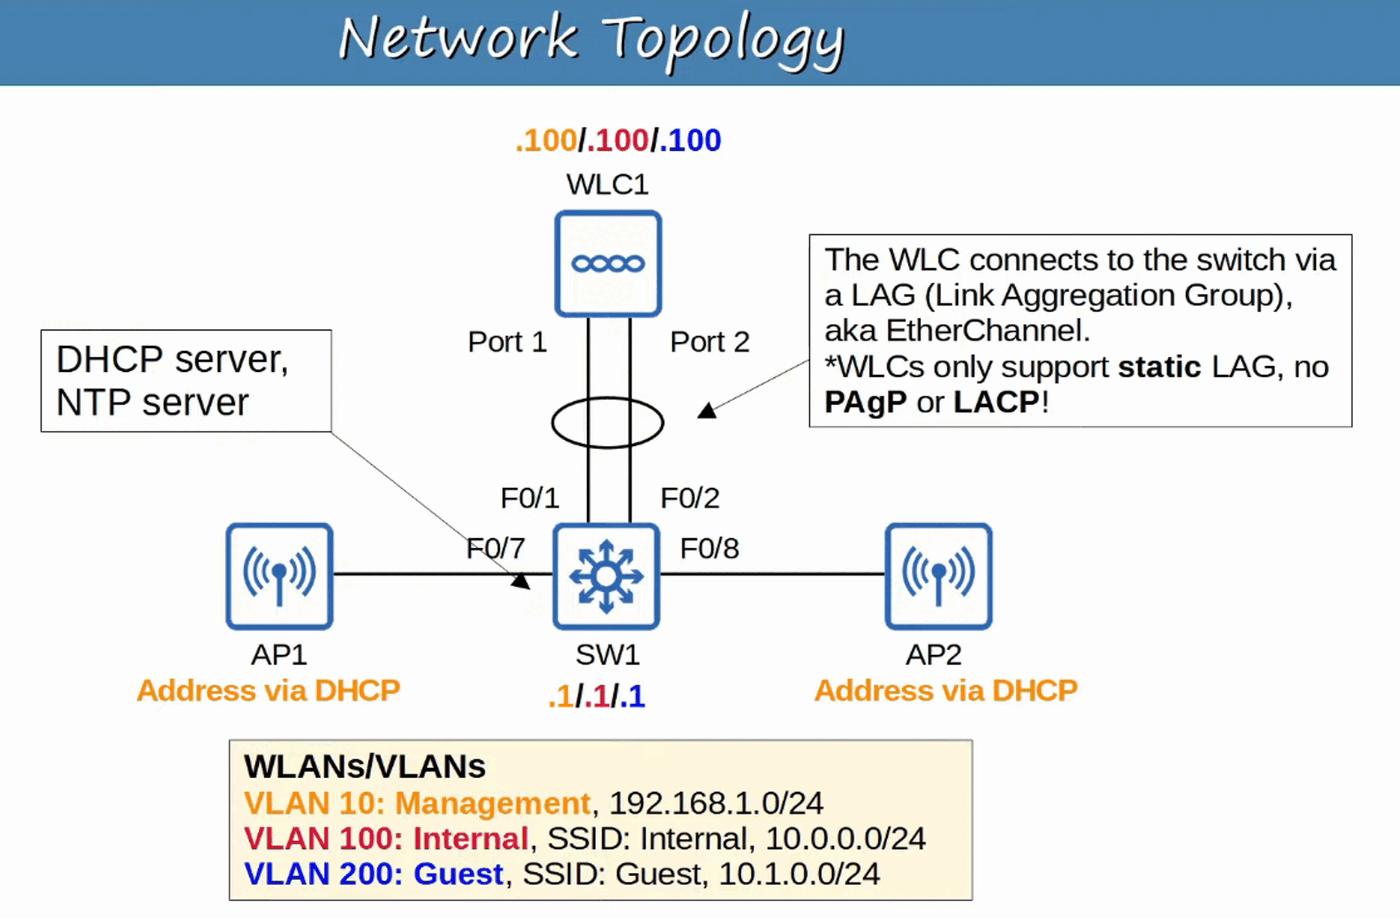
\includegraphics[keepaspectratio,alt={image}]{images/61-wireless-configuration/img-001.png}}
\end{figure}

INTERNAL PC (VLAN 100) ACCESSING DEFAULT GATEWAY via Internal CAPWAP
tunnel

\begin{figure}
\centering
\pandocbounded{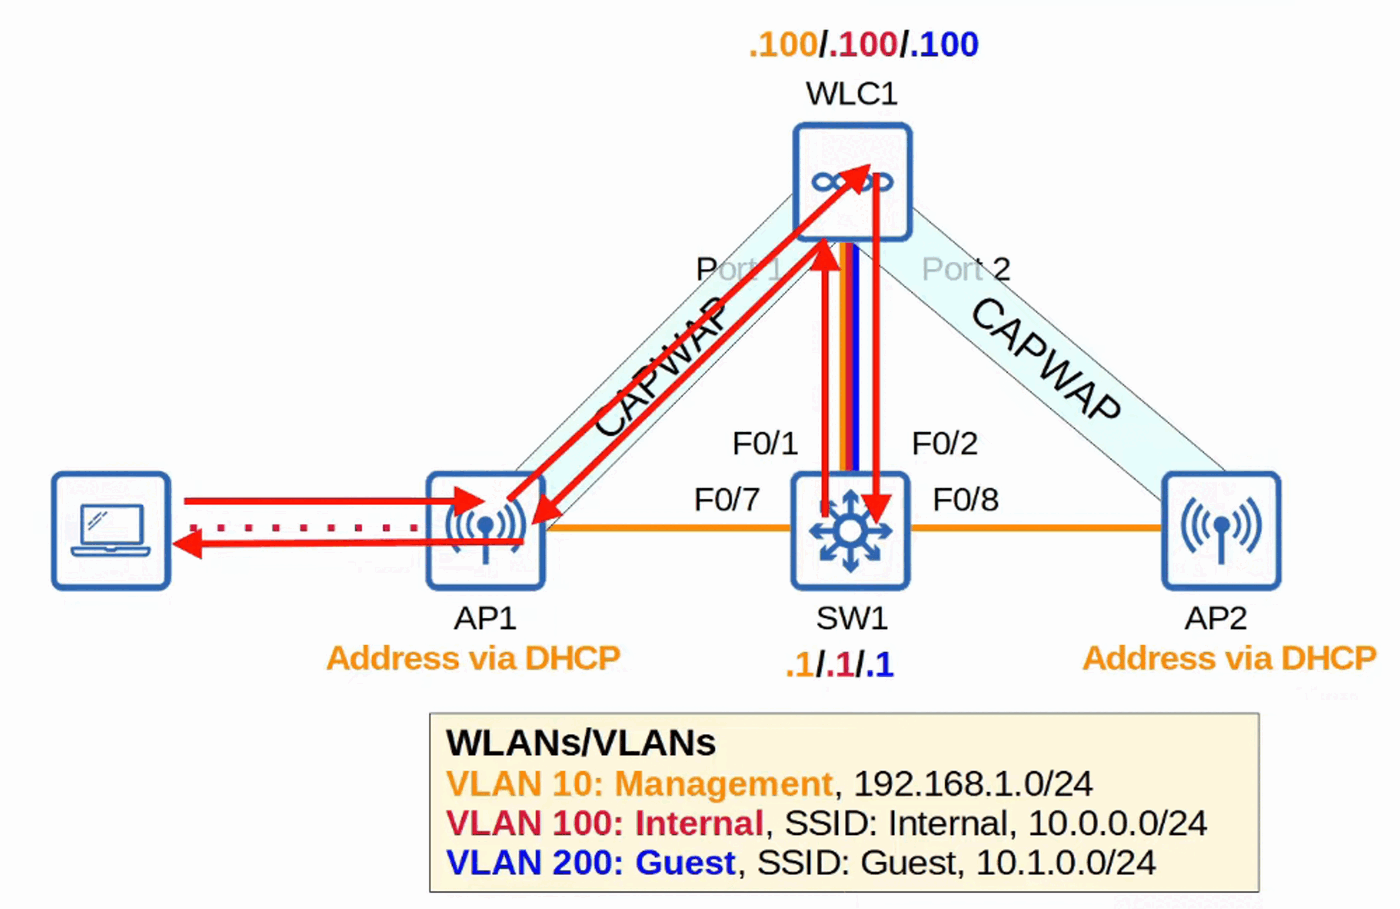
\includegraphics[keepaspectratio,alt={image}]{images/61-wireless-configuration/img-002.png}}
\end{figure}

REACHING External GUEST PC via DEFAULT GATEWAY + Internal and External
CAPWAP tunnels

\begin{figure}
\centering
\pandocbounded{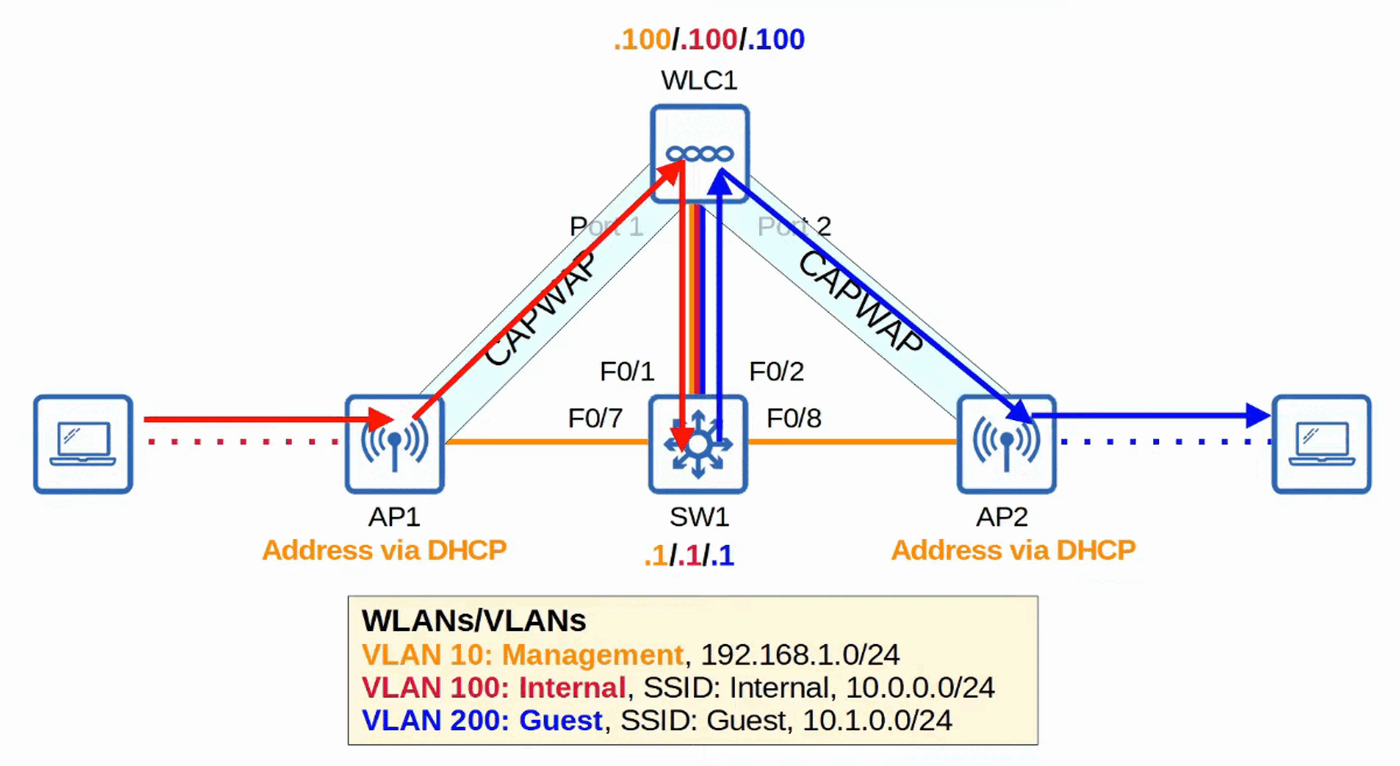
\includegraphics[keepaspectratio,alt={image}]{images/61-wireless-configuration/img-003.png}}
\end{figure}

\section{Layer 3 Switch Configuration
(SW1)}\label{layer-3-switch-configuration-sw1}

\begin{figure}
\centering
\pandocbounded{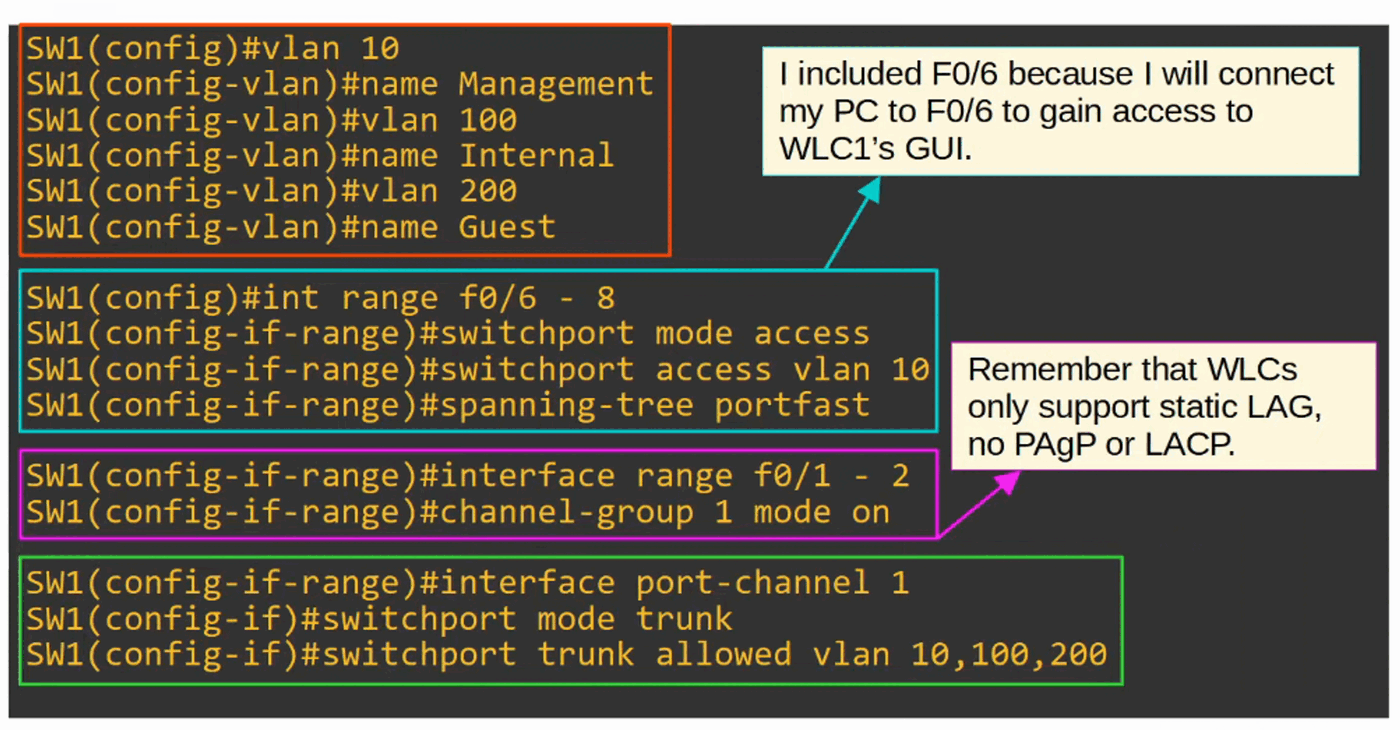
\includegraphics[keepaspectratio,alt={image}]{images/61-wireless-configuration/img-004.png}}
\end{figure}

PART 2 of configuration

Note DHCP ``Option 43''

\begin{figure}
\centering
\pandocbounded{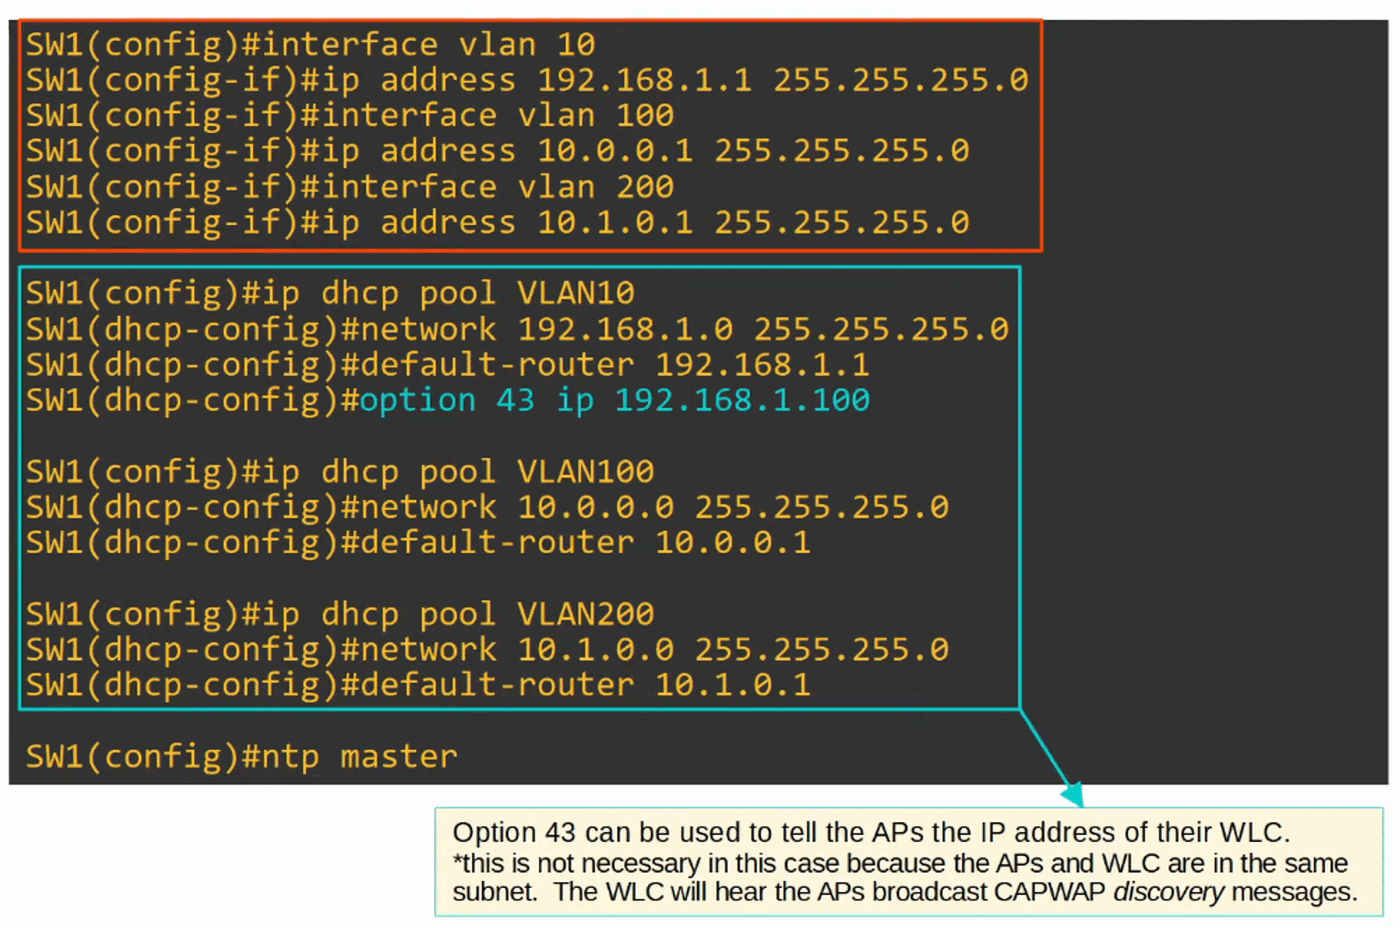
\includegraphics[keepaspectratio,alt={image}]{images/61-wireless-configuration/img-005.png}}
\end{figure}

\section{WLC Setup}\label{wlc-setup}

This helps set up the WLC to allow GUI configuration

\begin{figure}
\centering
\pandocbounded{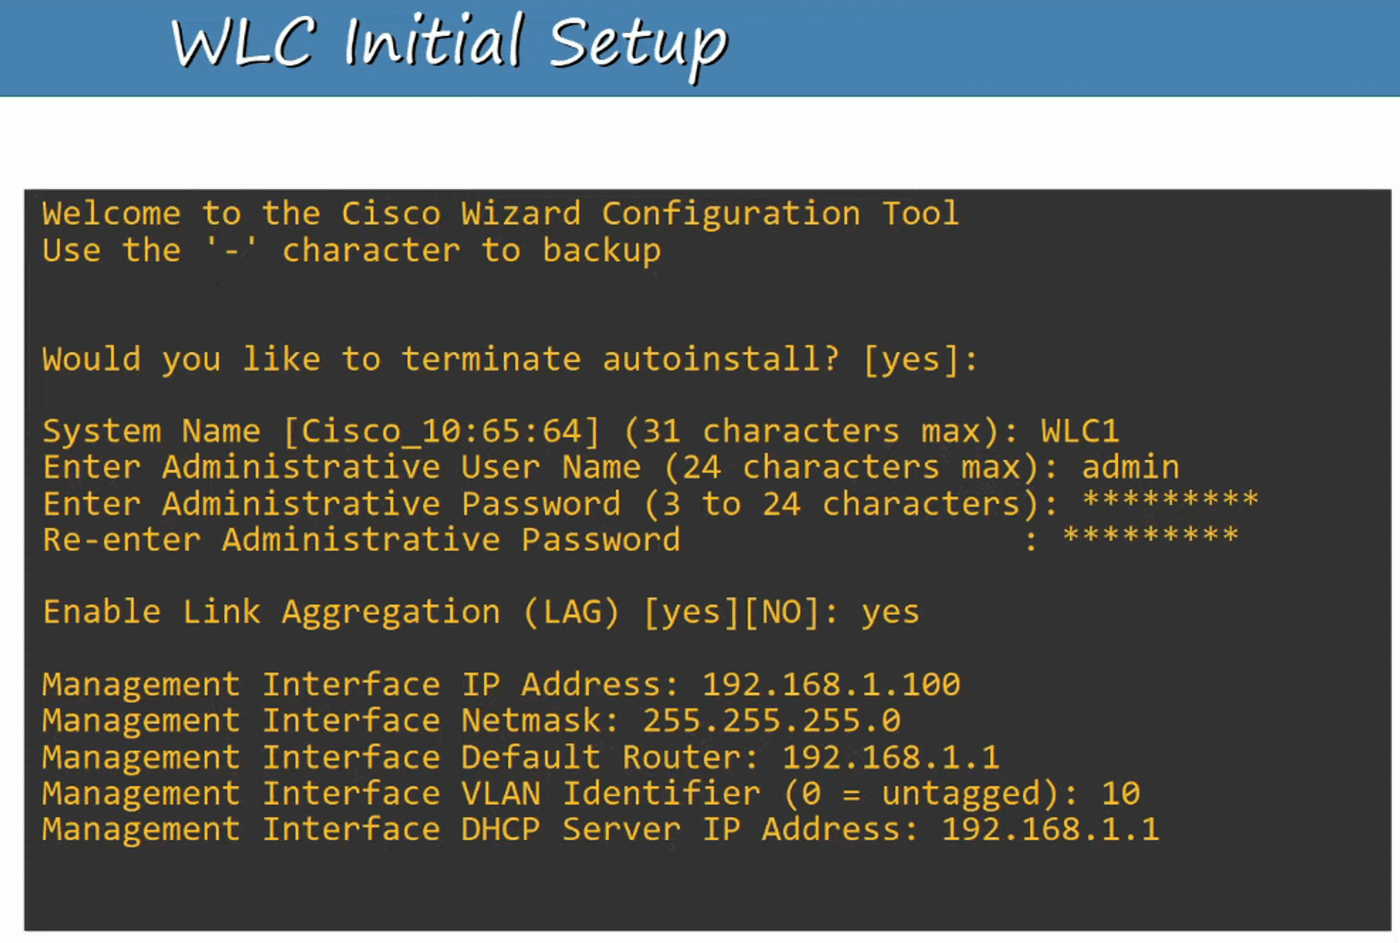
\includegraphics[keepaspectratio,alt={image}]{images/61-wireless-configuration/img-006.png}}
\end{figure}

\begin{figure}
\centering
\pandocbounded{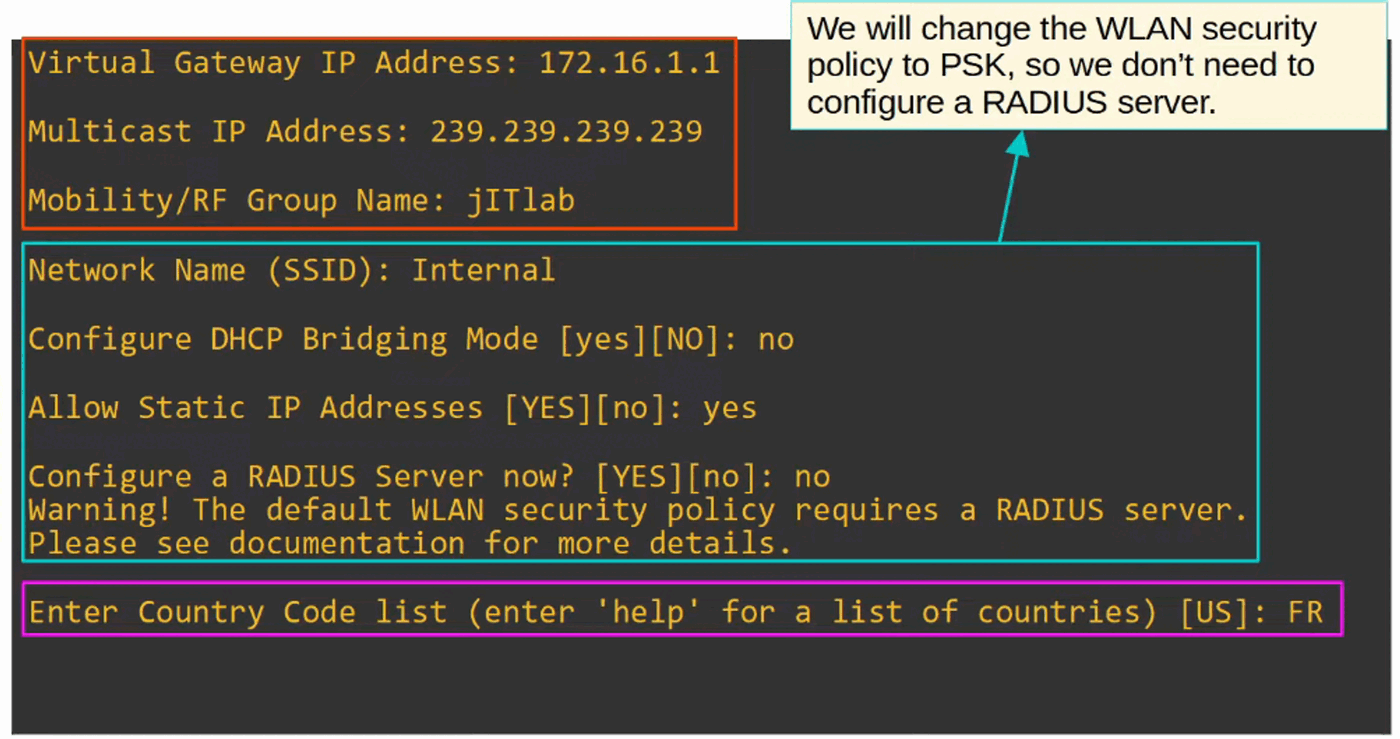
\includegraphics[keepaspectratio,alt={image}]{images/61-wireless-configuration/img-007.png}}
\end{figure}

Why Jeremy chose FRANCE for Country Code (has to do with regulatory
domain of equipment)

\begin{figure}
\centering
\pandocbounded{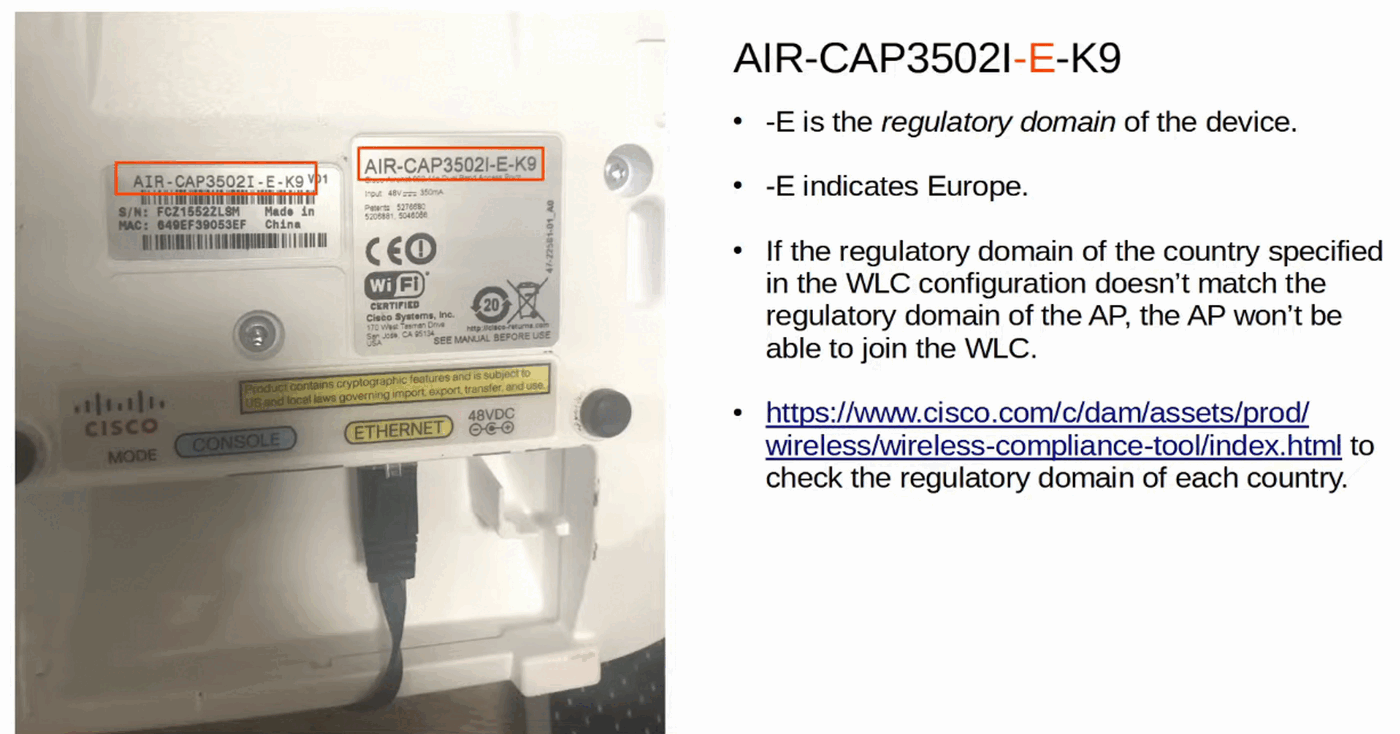
\includegraphics[keepaspectratio,alt={image}]{images/61-wireless-configuration/img-008.png}}
\end{figure}

\begin{figure}
\centering
\pandocbounded{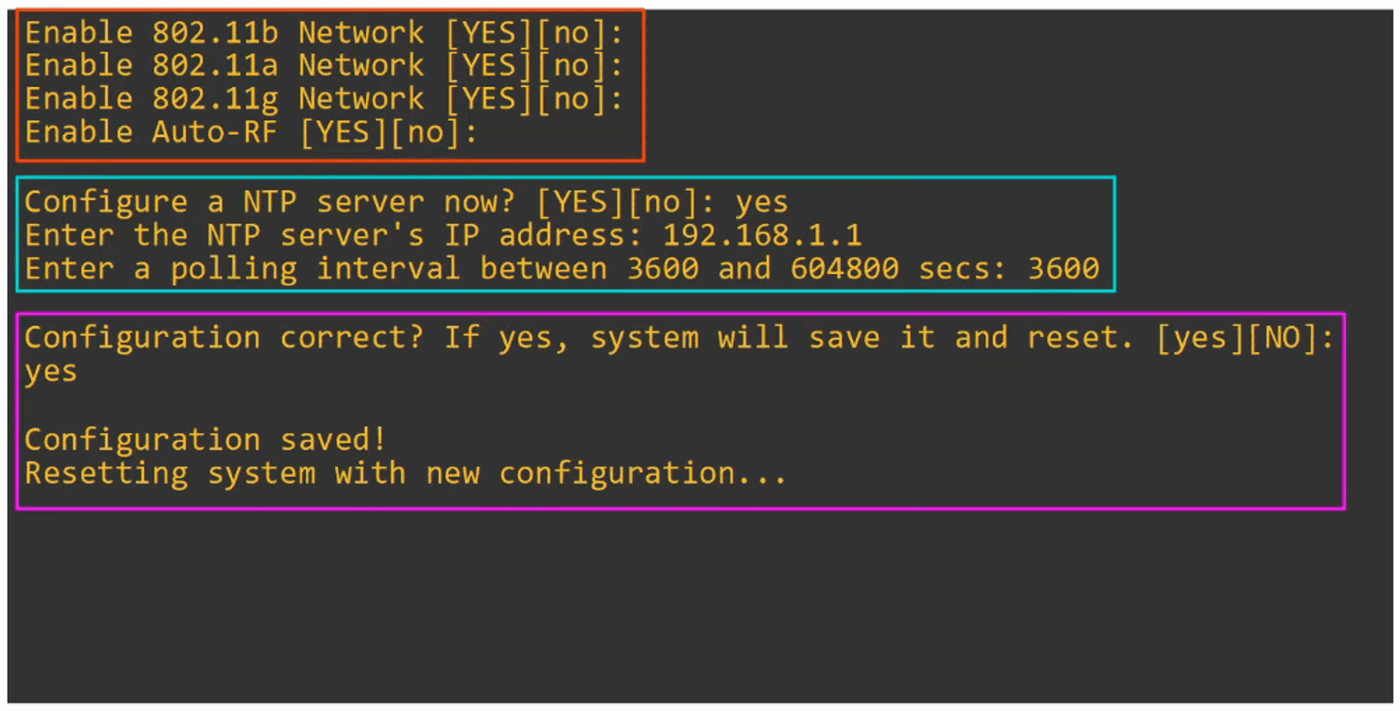
\includegraphics[keepaspectratio,alt={image}]{images/61-wireless-configuration/img-009.png}}
\end{figure}

\section{Accessing the WLC GUI}\label{accessing-the-wlc-gui}

\begin{figure}
\centering
\pandocbounded{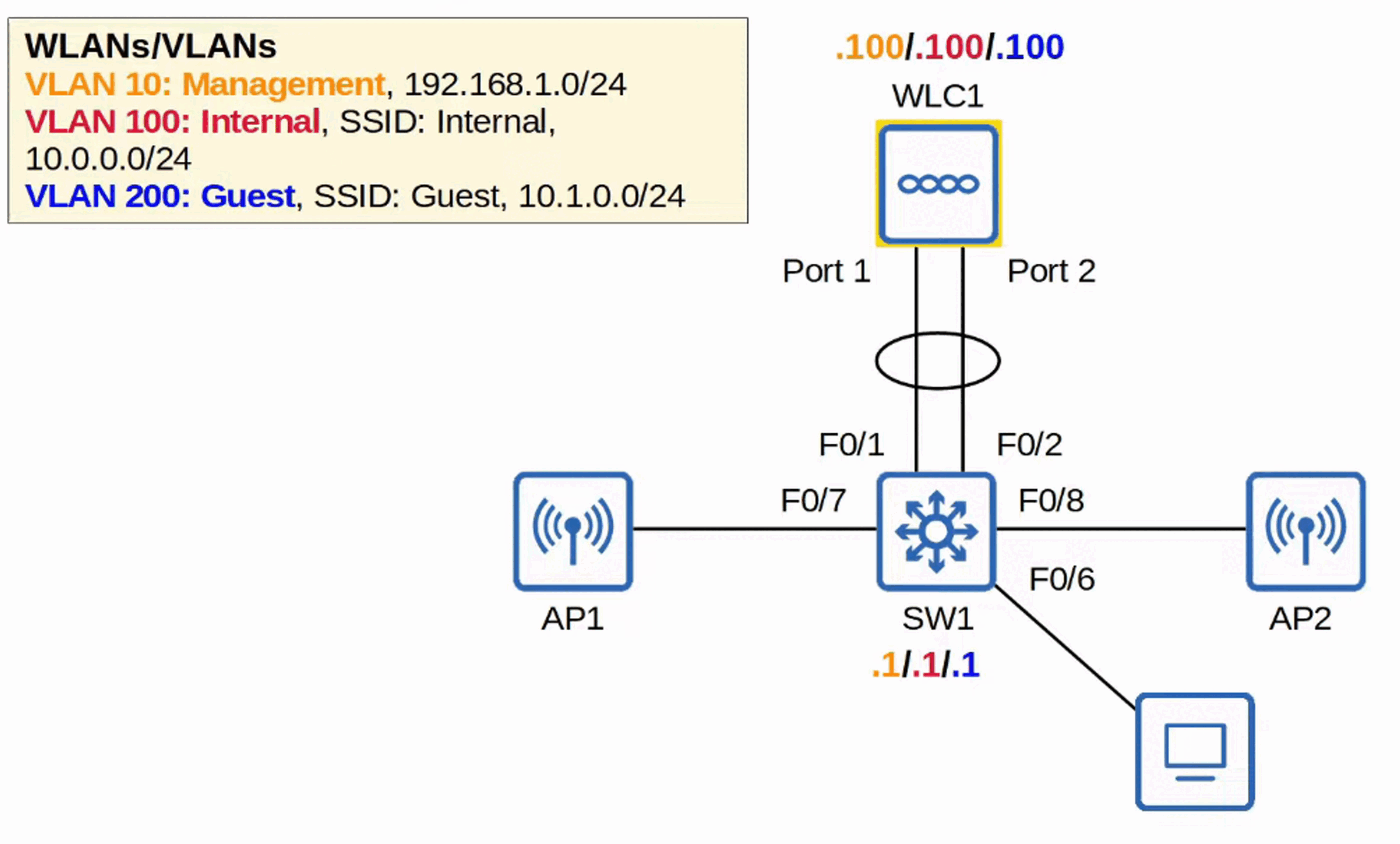
\includegraphics[keepaspectratio,alt={image}]{images/61-wireless-configuration/img-010.png}}
\end{figure}

\begin{figure}
\centering
\pandocbounded{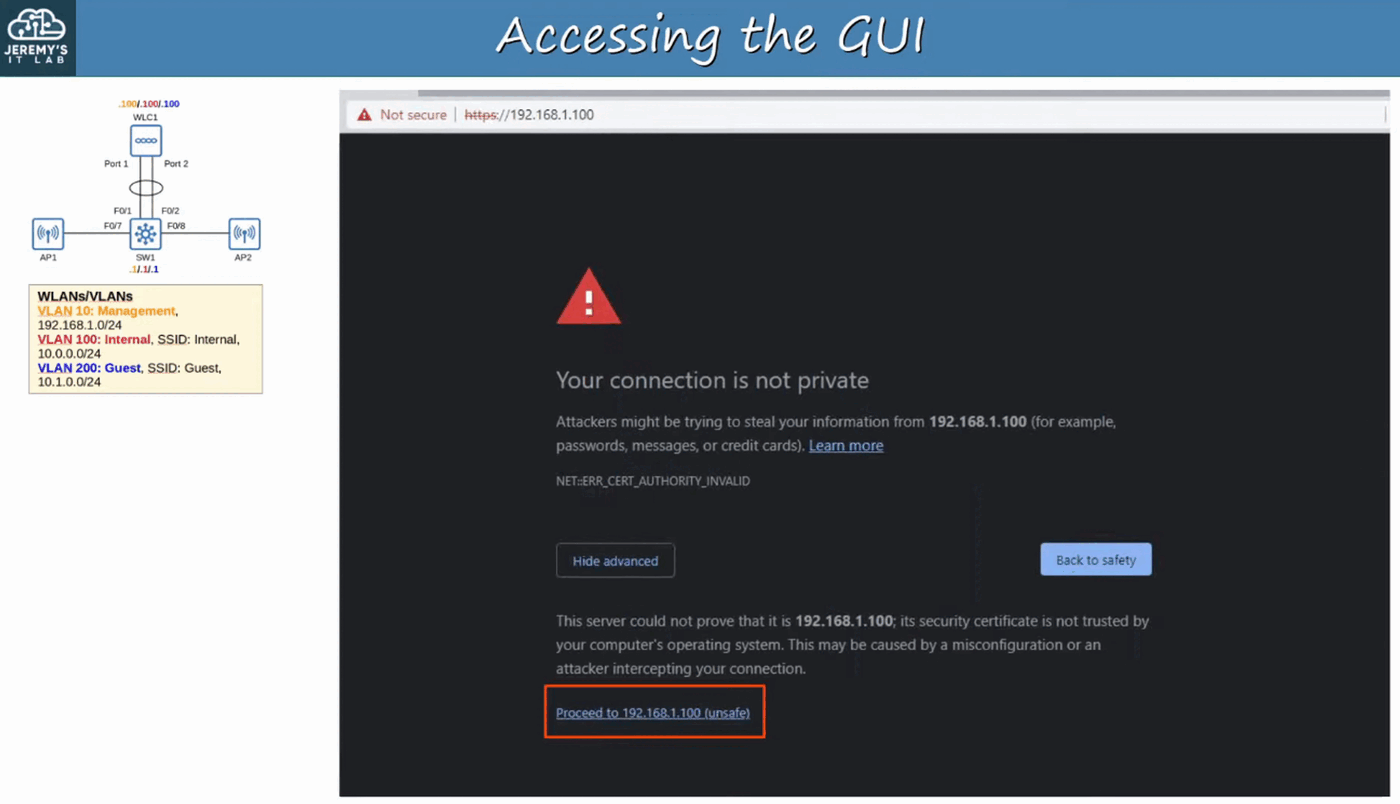
\includegraphics[keepaspectratio,alt={image}]{images/61-wireless-configuration/img-011.png}}
\end{figure}

\begin{figure}
\centering
\pandocbounded{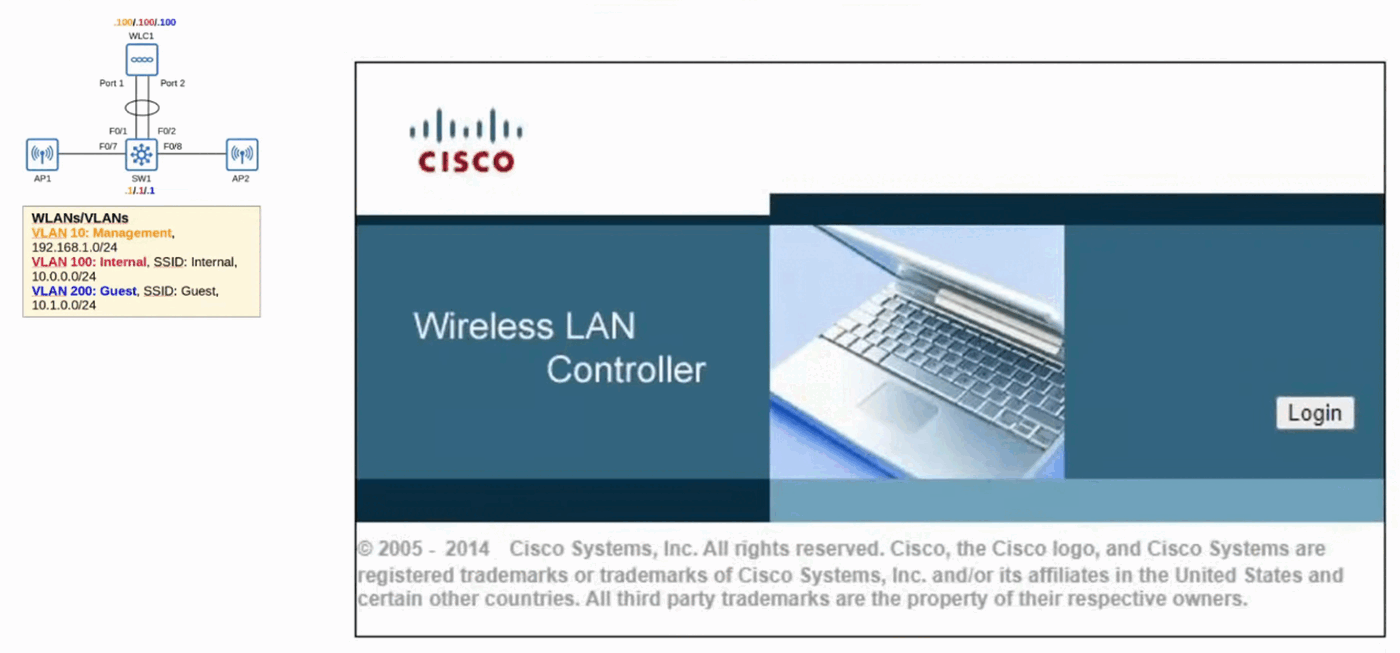
\includegraphics[keepaspectratio,alt={image}]{images/61-wireless-configuration/img-012.png}}
\end{figure}

\begin{figure}
\centering
\pandocbounded{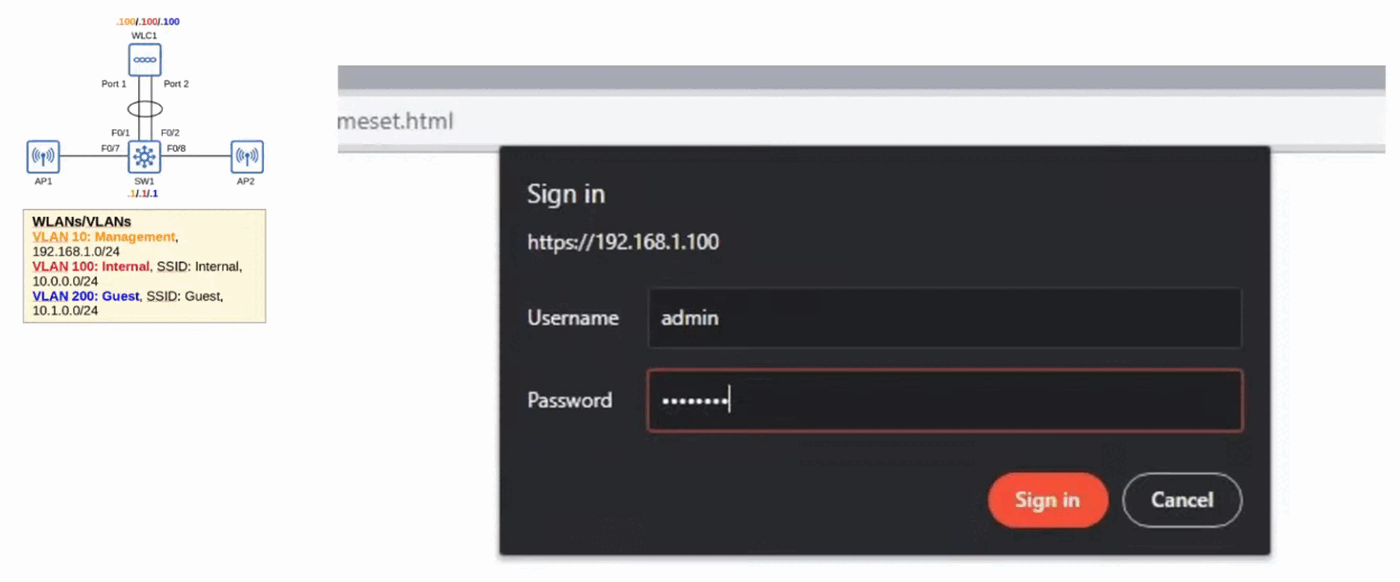
\includegraphics[keepaspectratio,alt={image}]{images/61-wireless-configuration/img-013.png}}
\end{figure}

\begin{figure}
\centering
\pandocbounded{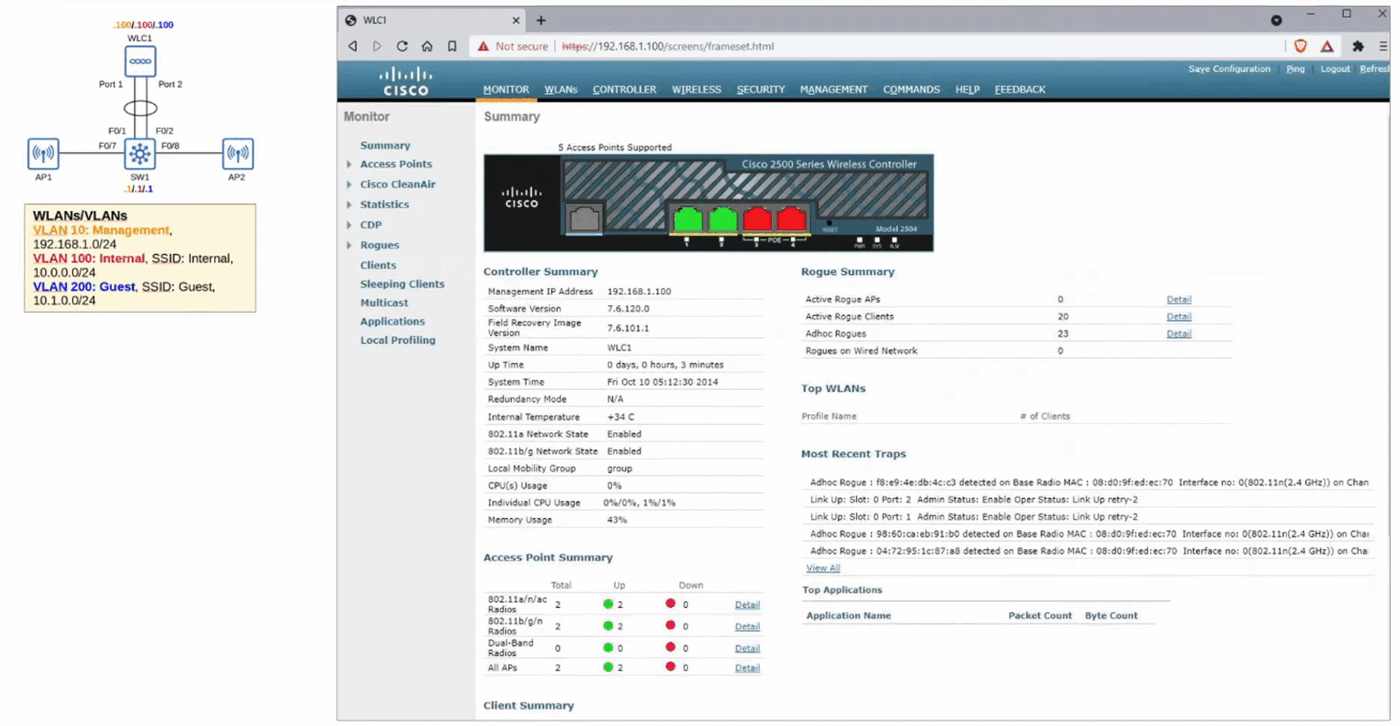
\includegraphics[keepaspectratio,alt={image}]{images/61-wireless-configuration/img-014.png}}
\end{figure}

\section{WLC Configuration}\label{wlc-configuration}

\begin{figure}
\centering
\pandocbounded{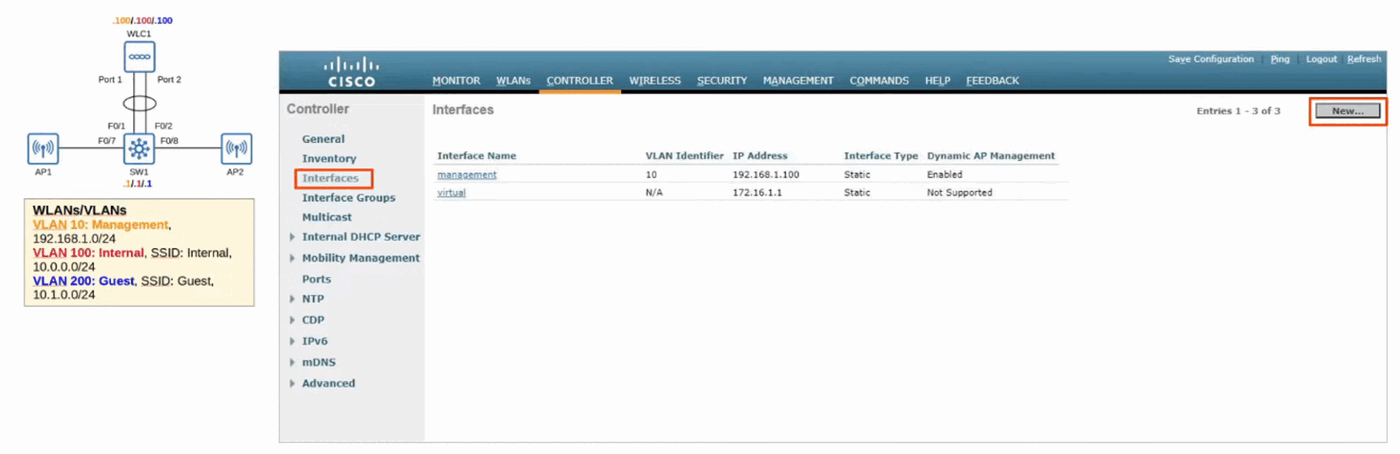
\includegraphics[keepaspectratio,alt={image}]{images/61-wireless-configuration/img-015.png}}
\end{figure}

\section{WLC Ports}\label{wlc-ports}

\begin{itemize}
\tightlist
\item
  WLC PORTS are the PHYSICAL PORTS that cables connect to
\item
  WLC INTERFACES are the logical interfaces within the WLC (ie: SVIs on
  a SWITCH)
\item
  WLCs have a few different PORTS:

  \begin{itemize}
  \tightlist
  \item
    SERVICE PORT

    \begin{itemize}
    \tightlist
    \item
      A dedicated MANAGEMENT PORT
    \item
      Used for OUT-OF-BAND management
    \item
      Must connected to a SWITCH ACCESS PORT because it only supports
      one VLAN
    \item
      This PORT can be used to connect to the DEVICE while it is
      booting, performing system recovery, etc.
    \end{itemize}
  \item
    DISTRIBUTION SYSTEM PORT

    \begin{itemize}
    \tightlist
    \item
      These are the standard NETWORK PORTS that connect to the
      ``DISTRIBUTION SYSTEM'' (WIRED NETWORK) and are used for DATA
      traffic.
    \item
      These PORTS usually connect to SWITCH TRUNK PORTS, and if multiple
      distribution PORTS are used they can form a LAG
    \end{itemize}
  \item
    CONSOLE PORT

    \begin{itemize}
    \tightlist
    \item
      This is a standard CONSOLE PORT, either RJ45 or USB
    \end{itemize}
  \item
    REDUNDANCY PORT

    \begin{itemize}
    \tightlist
    \item
      This PORT is used to connect to another WLC to form a HIGH
      AVAILABILITY (HA) pair
    \end{itemize}
  \end{itemize}
\end{itemize}

\begin{figure}
\centering
\pandocbounded{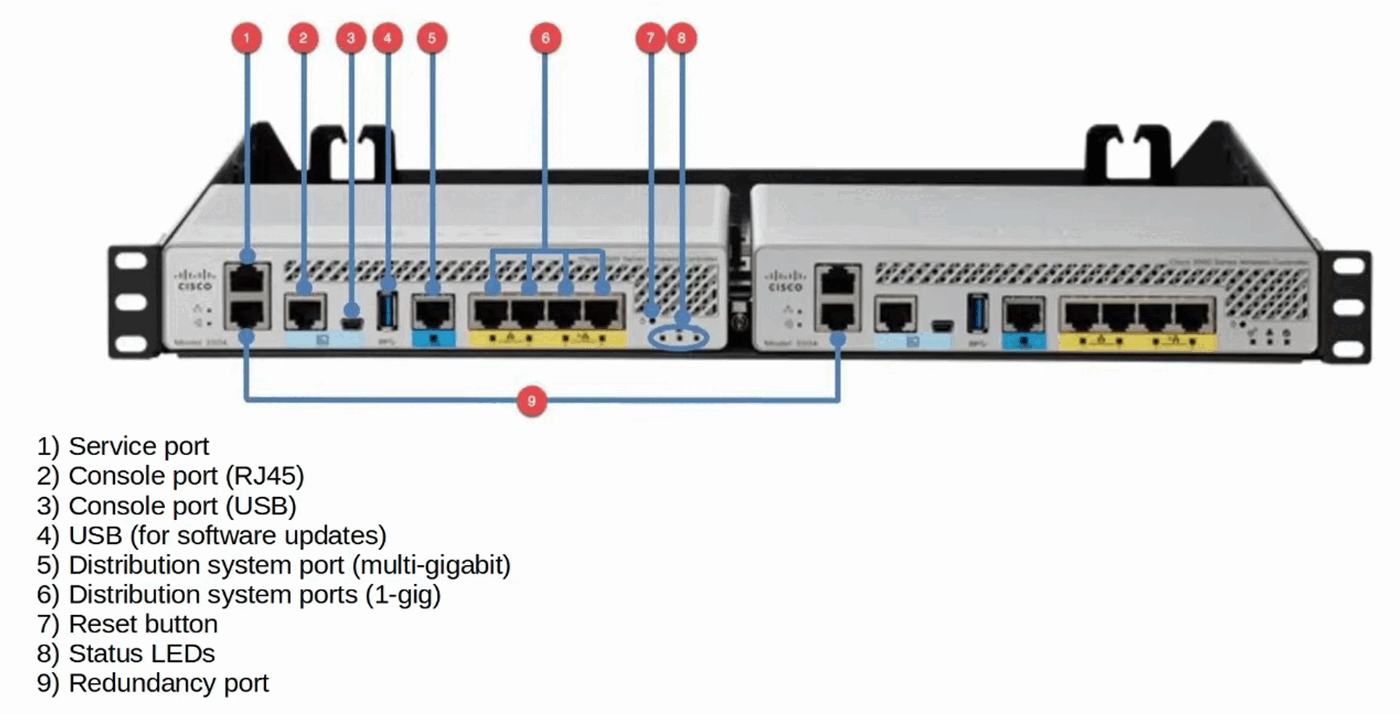
\includegraphics[keepaspectratio,alt={image}]{images/61-wireless-configuration/img-016.png}}
\end{figure}

\section{WLC Interfaces}\label{wlc-interfaces}

\begin{itemize}
\tightlist
\item
  MANAGEMENT INTERFACES

  \begin{itemize}
  \tightlist
  \item
    Used for management traffic such as TELNET, SSH, HTTP, HTTPS, RADIUS
    authentication, NTP, SYSLOG, etc.
  \item
    CAPWAP TUNNELS are also formed to / from the WLC's management
    INTERFACE
  \end{itemize}
\item
  REDUNDANCY MANAGEMENT INTERFACE

  \begin{itemize}
  \tightlist
  \item
    When TWO WLCs are connected by their REDUNDANCY PORTS, one WLC is
    ``ACTIVE'' and the other is ``STANDBY''
  \item
    This INTERFACE can be used to connect to and manage the ``STANDBY''
    WLC
  \end{itemize}
\item
  VIRTUAL INTERFACE

  \begin{itemize}
  \tightlist
  \item
    This INTERFACE is used when communicating with WIRELESS CLIENTS to
    relay DHCP requests, perform CLIENT WEB AUTHENTICATION, etc.
  \end{itemize}
\item
  SERVICE PORT INTERFACE

  \begin{itemize}
  \tightlist
  \item
    If the SERVICE PORT is used, this INTERFACE is bound to it and used
    for OUT-OF-BAND MANAGEMENT
  \end{itemize}
\item
  DYNAMIC INTERFACE

  \begin{itemize}
  \tightlist
  \item
    These are the INTERFACES used to map a WLAN to a VLAN
  \item
    For example :

    \begin{itemize}
    \tightlist
    \item
      TRAFFIC from the ``INTERNAL'' WLAN will be sent to the WIRED
      NETWORK from the WLCs ``INTERNAL'' DYNAMIC INTERFACE
    \end{itemize}
  \end{itemize}
\end{itemize}

\section{WLAN Configuration}\label{wlan-configuration}

Click ``NEW''

\begin{figure}
\centering
\pandocbounded{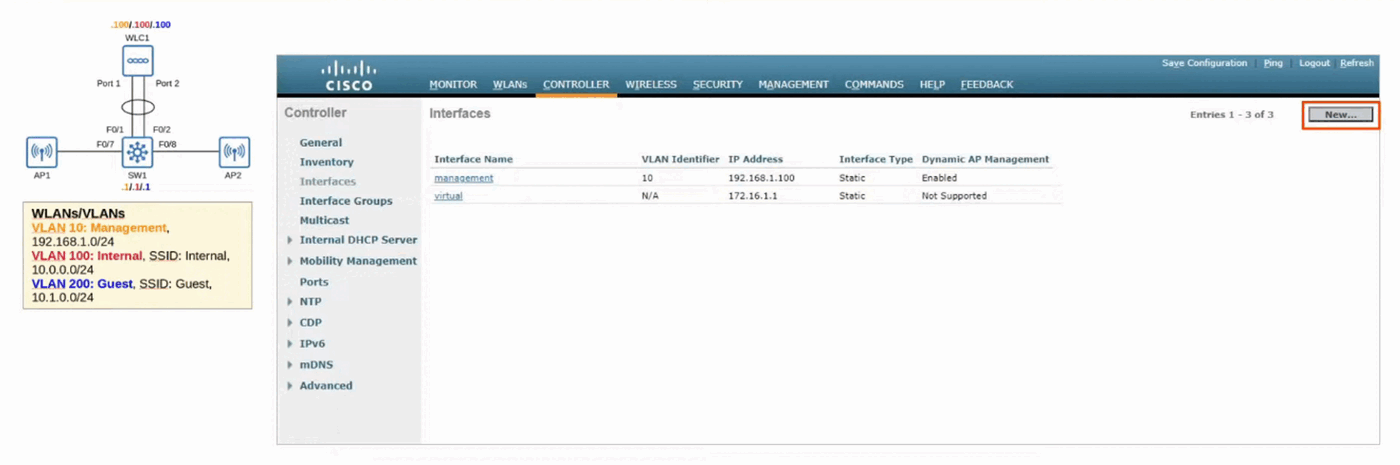
\includegraphics[keepaspectratio,alt={image}]{images/61-wireless-configuration/img-017.png}}
\end{figure}

Fill in details of the interface and click ``APPLY''

\begin{figure}
\centering
\pandocbounded{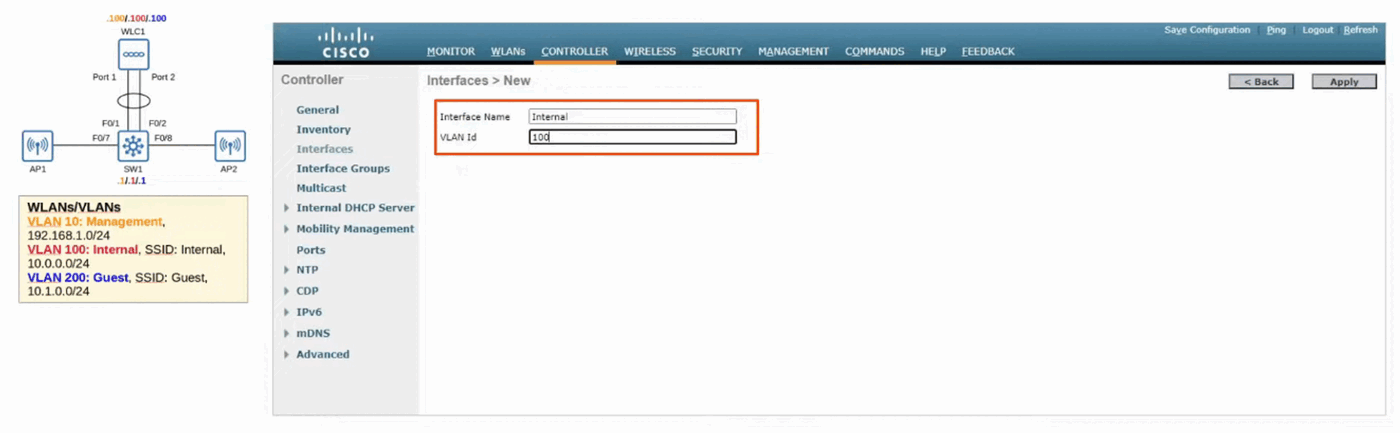
\includegraphics[keepaspectratio,alt={image}]{images/61-wireless-configuration/img-018.png}}
\end{figure}

Fill out details (IP, Netmask, Gateway\ldots) and then click ``APPLY''

\begin{figure}
\centering
\pandocbounded{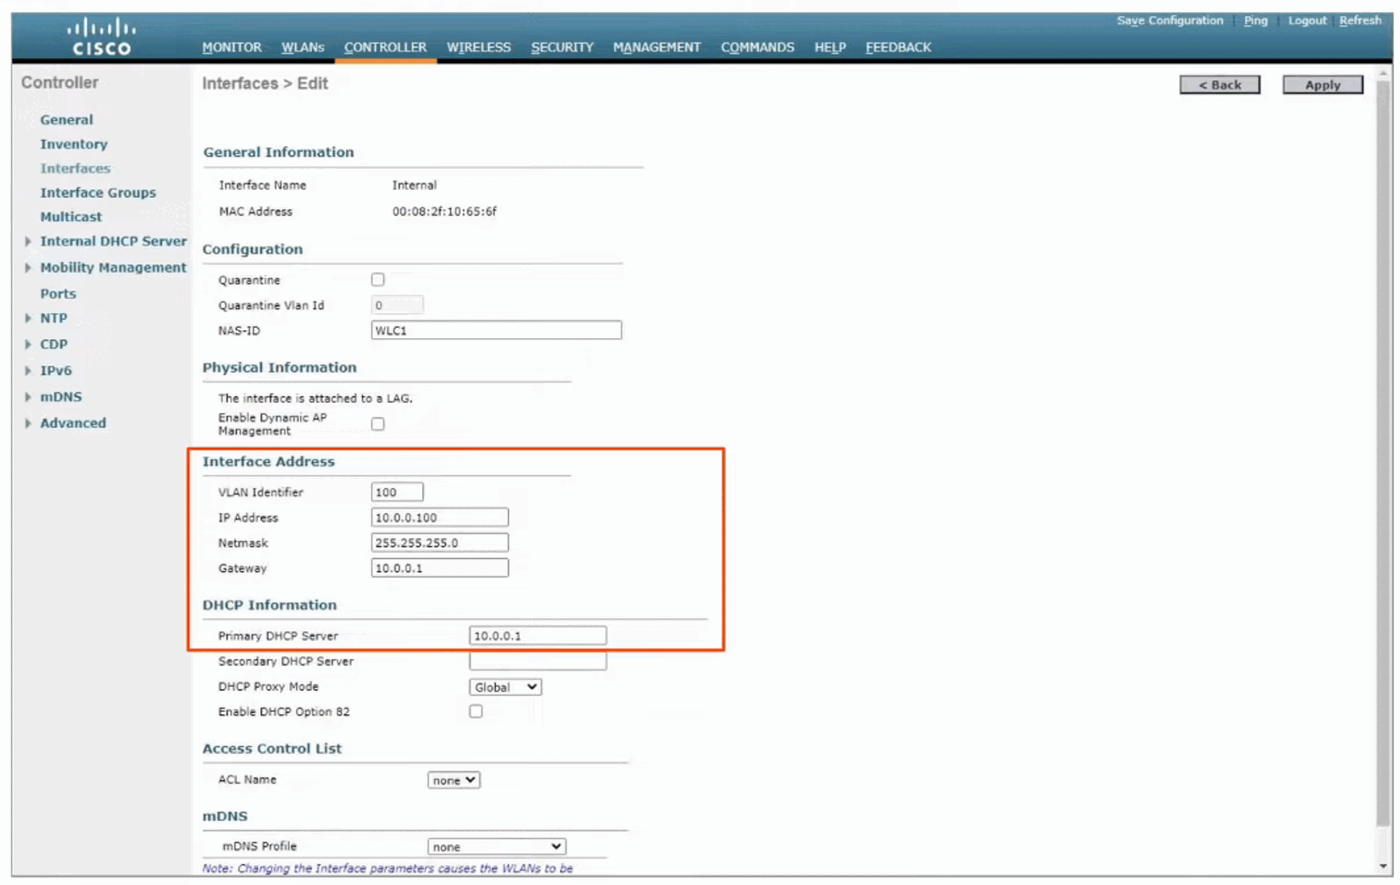
\includegraphics[keepaspectratio,alt={image}]{images/61-wireless-configuration/img-019.png}}
\end{figure}

INTERNAL interface has now been created

\begin{figure}
\centering
\pandocbounded{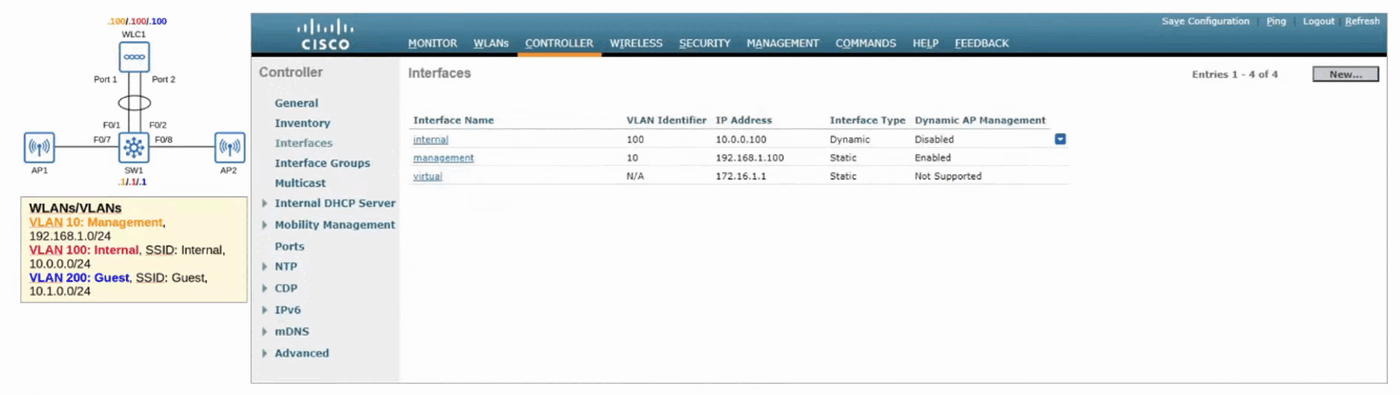
\includegraphics[keepaspectratio,alt={image}]{images/61-wireless-configuration/img-020.png}}
\end{figure}

Now, repeat the above steps for the GUEST interface

\begin{figure}
\centering
\pandocbounded{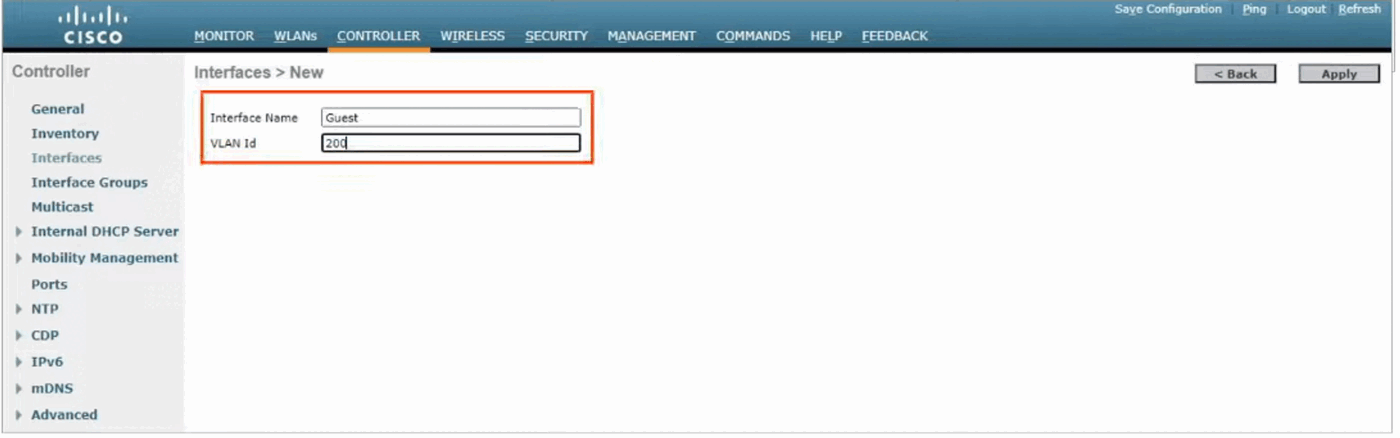
\includegraphics[keepaspectratio,alt={image}]{images/61-wireless-configuration/img-021.png}}
\end{figure}

Fill out details (IP, Netmask, Gateway\ldots) and then click ``APPLY''

\begin{figure}
\centering
\pandocbounded{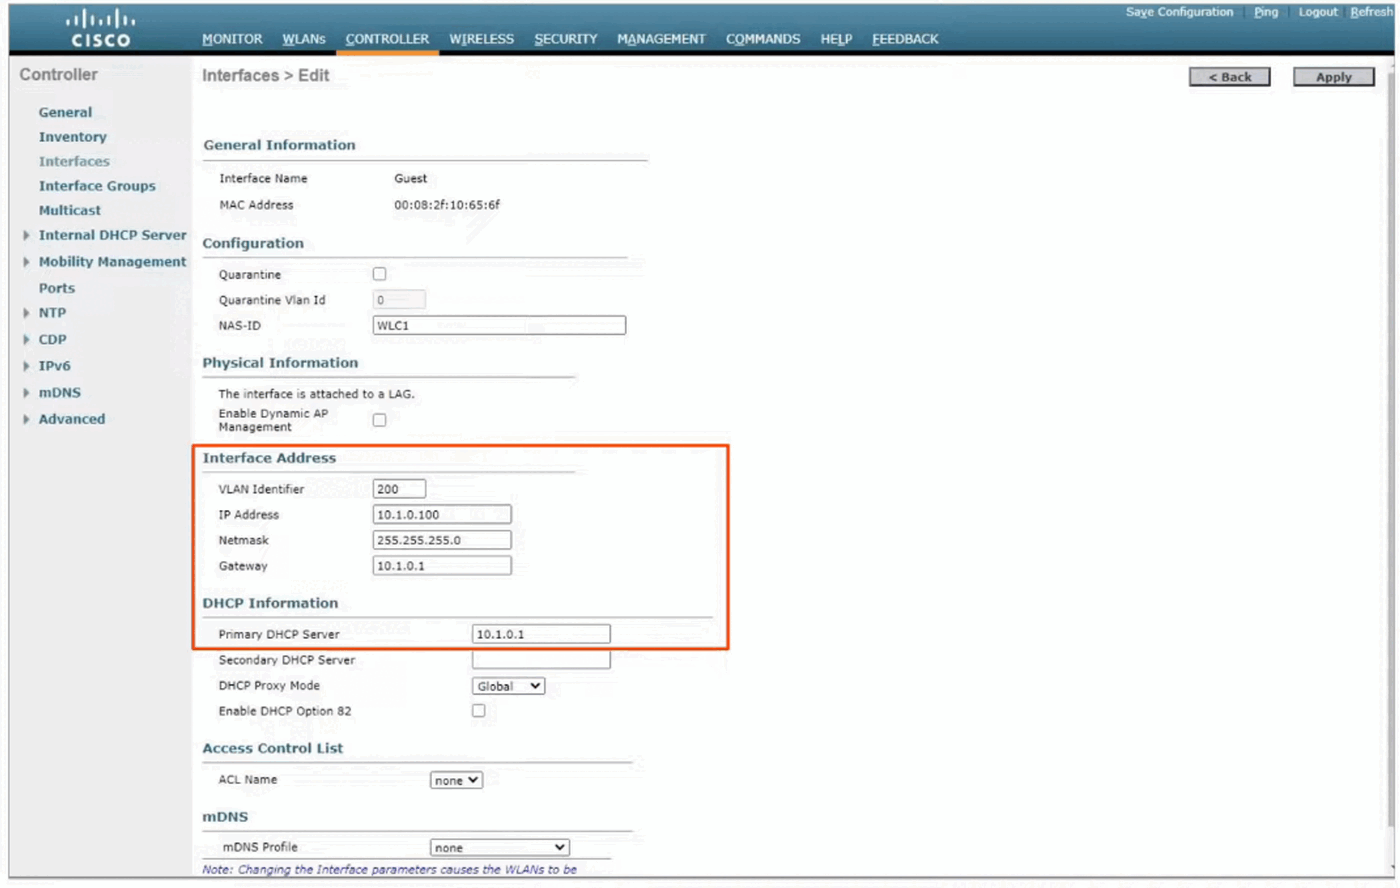
\includegraphics[keepaspectratio,alt={image}]{images/61-wireless-configuration/img-022.png}}
\end{figure}

\begin{figure}
\centering
\pandocbounded{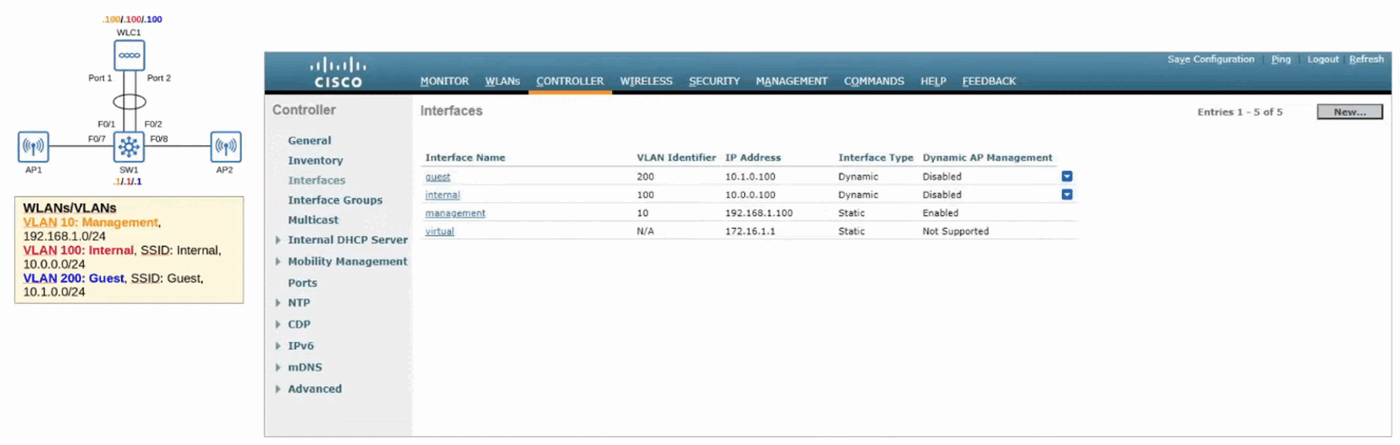
\includegraphics[keepaspectratio,alt={image}]{images/61-wireless-configuration/img-023.png}}
\end{figure}

Now that all the INTERFACES are created, we can start WLAN CONFIGURATION

\begin{figure}
\centering
\pandocbounded{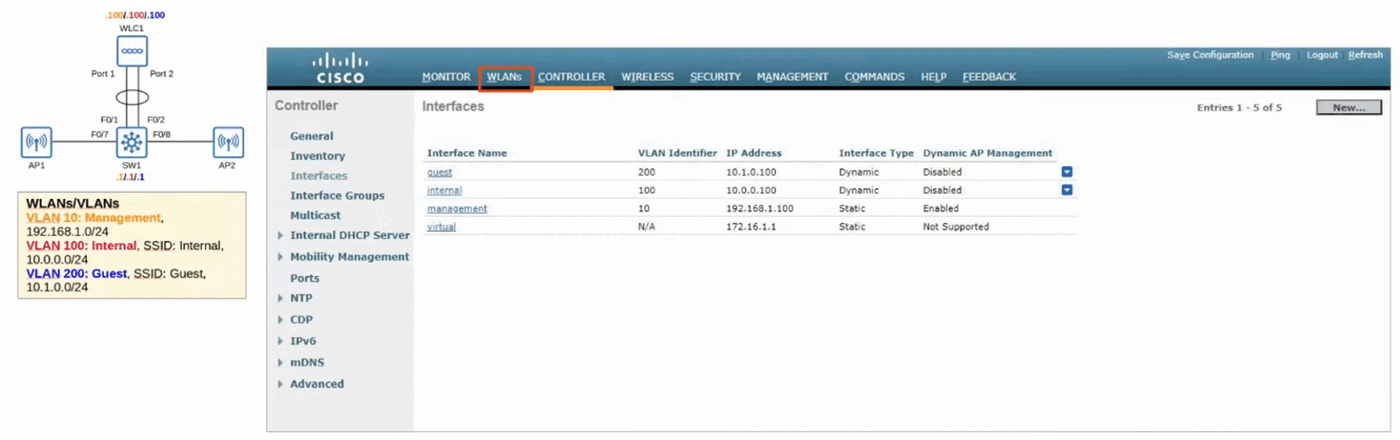
\includegraphics[keepaspectratio,alt={image}]{images/61-wireless-configuration/img-024.png}}
\end{figure}

\begin{figure}
\centering
\pandocbounded{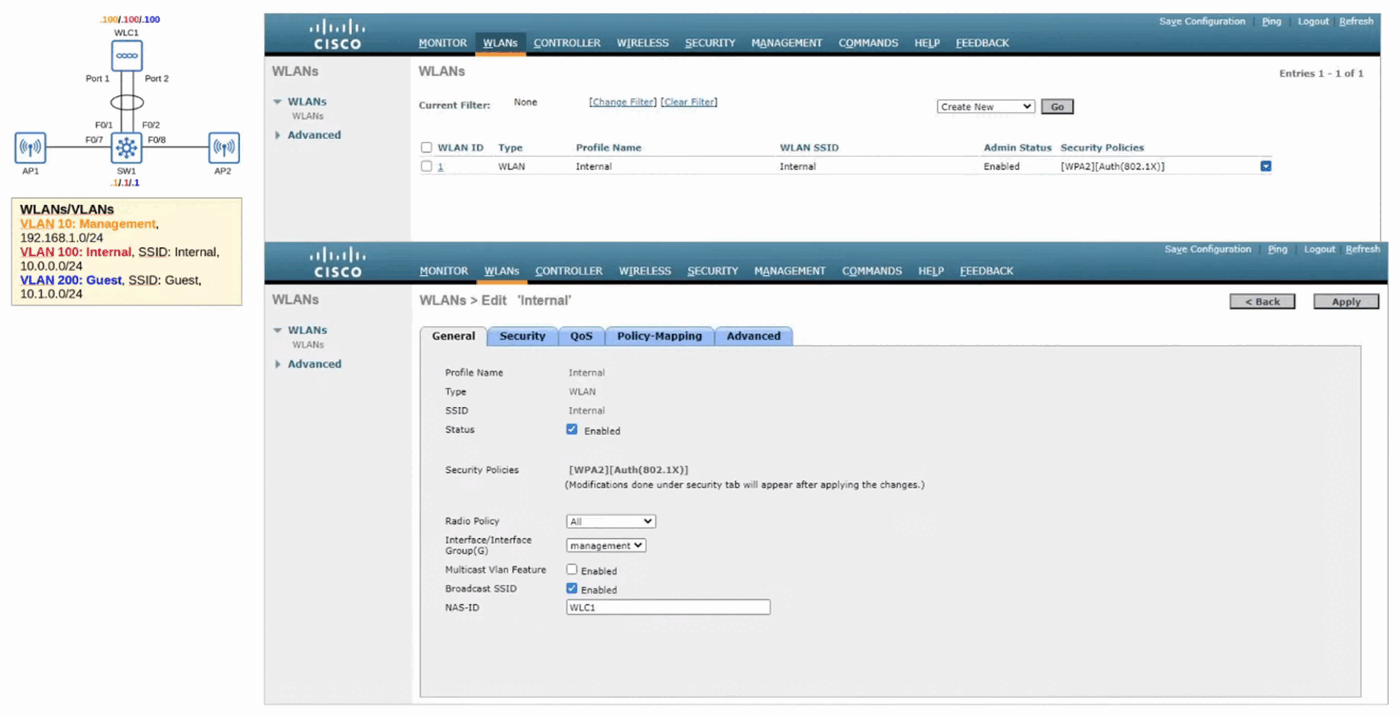
\includegraphics[keepaspectratio,alt={image}]{images/61-wireless-configuration/img-025.png}}
\end{figure}

INTERNAL WLAN is set to ``MANAGEMENT'', it needs to be changed to
``INTERNAL''

\begin{figure}
\centering
\pandocbounded{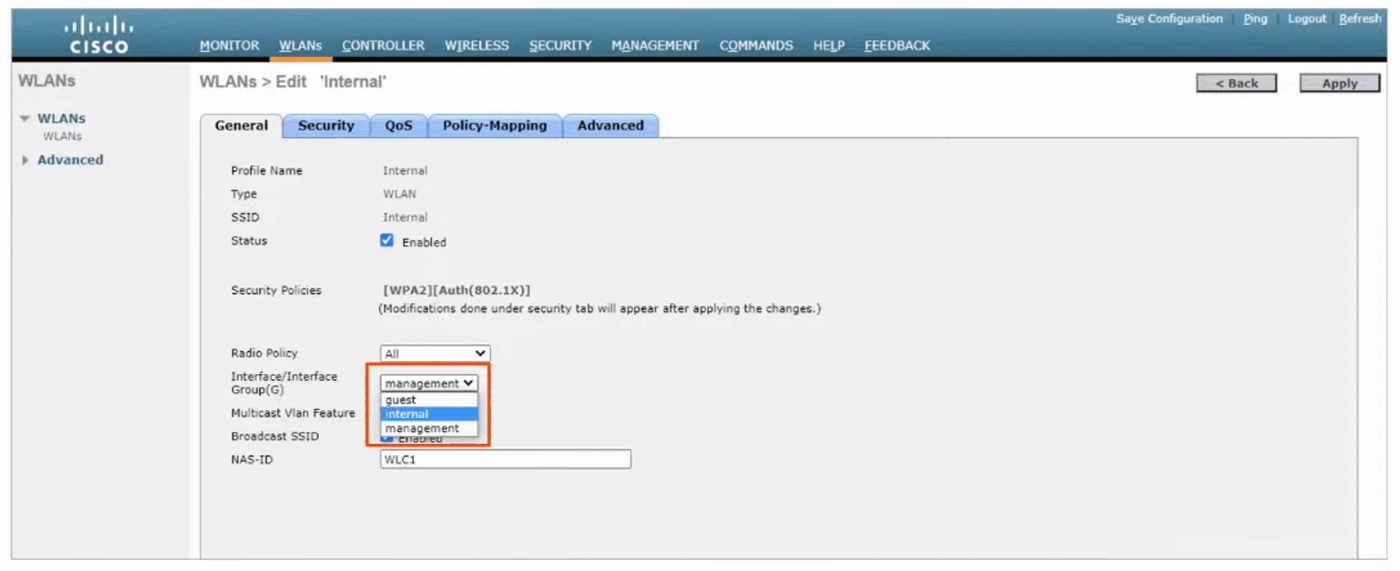
\includegraphics[keepaspectratio,alt={image}]{images/61-wireless-configuration/img-026.png}}
\end{figure}

SECURITY will also need to be changed from {[}WPA2{]} to {[}WPA2 PSK{]}

\begin{figure}
\centering
\pandocbounded{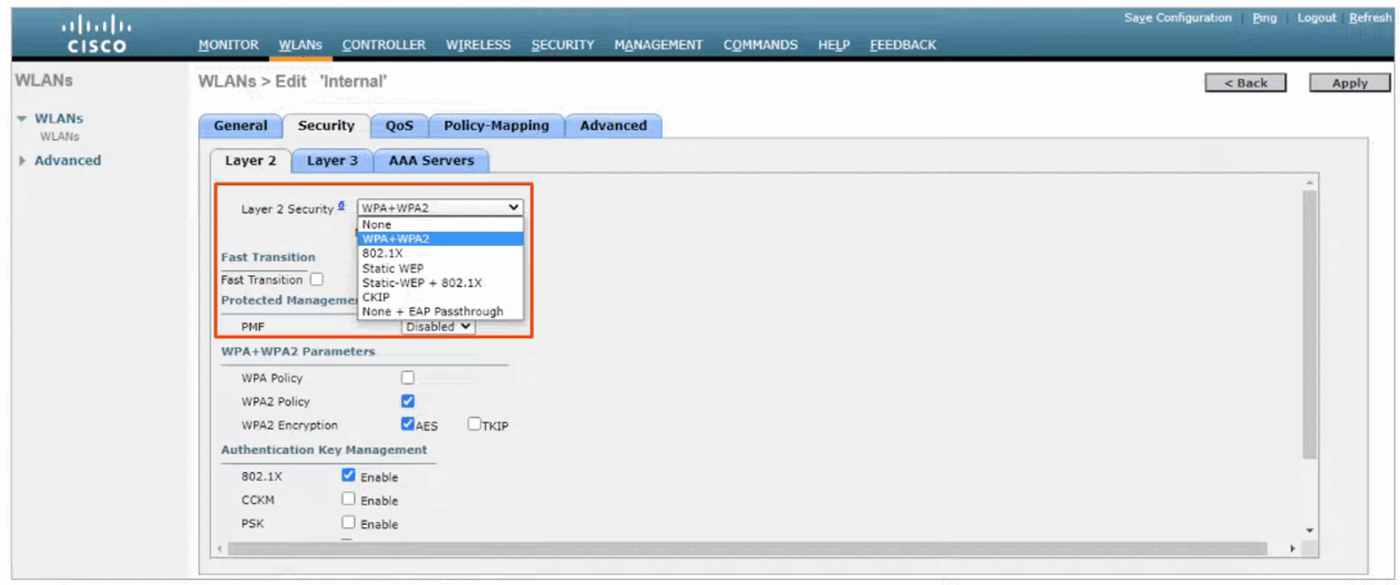
\includegraphics[keepaspectratio,alt={image}]{images/61-wireless-configuration/img-027.png}}
\end{figure}

(Need to CHECK the PSK ``Enable'' box at the bottom)

Change the PSK FORMAT to ``ASCII'' and enter a PASSWORD (at least 8
chars in length)

\begin{figure}
\centering
\pandocbounded{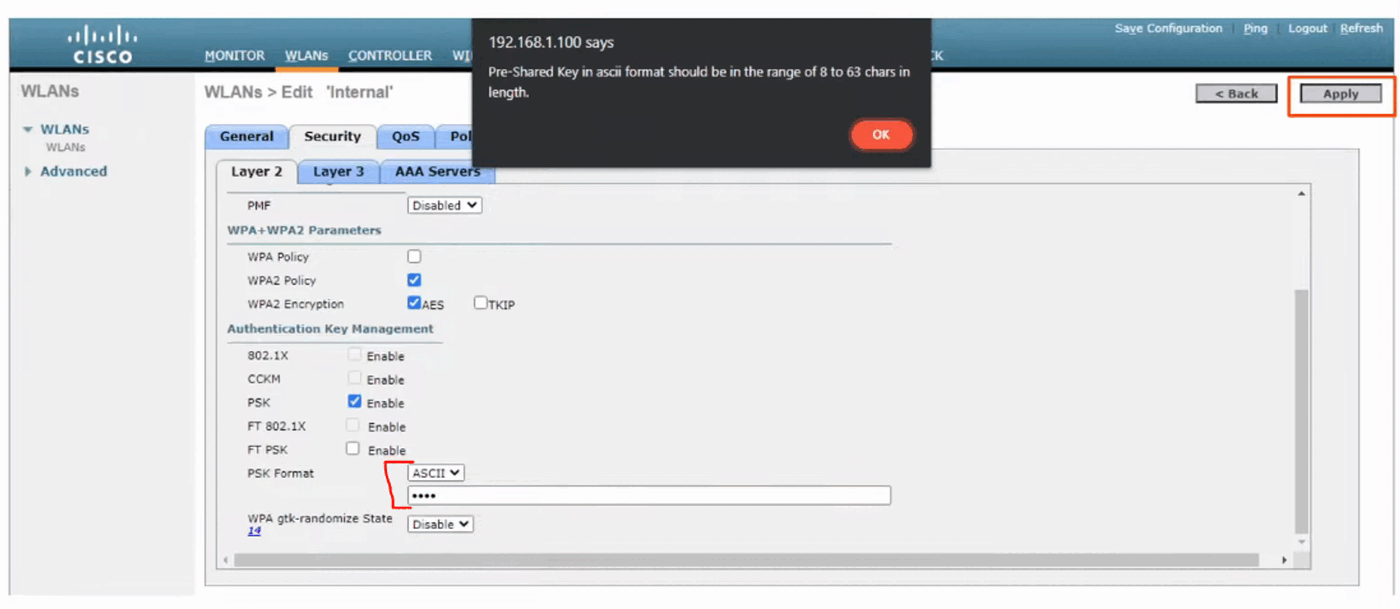
\includegraphics[keepaspectratio,alt={image}]{images/61-wireless-configuration/img-028.png}}
\end{figure}

\begin{figure}
\centering
\pandocbounded{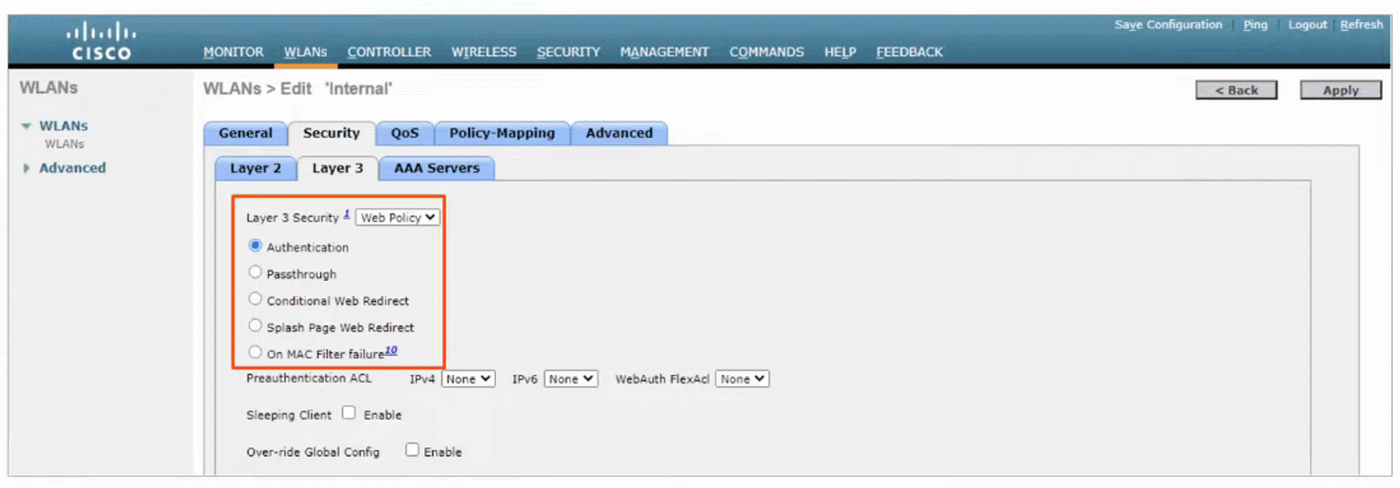
\includegraphics[keepaspectratio,alt={image}]{images/61-wireless-configuration/img-029.png}}
\end{figure}

\begin{itemize}
\tightlist
\item
  WEB AUTHENTICATION

  \begin{itemize}
  \tightlist
  \item
    After the WIRELESS CLIENTS gets an IP ADDRESS and tries to access a
    WEB PAGE, they will have to enter a USERNAME and PASSWORD to
    AUTHENTICATE
  \end{itemize}
\item
  WEB PASSTHROUGH

  \begin{itemize}
  \tightlist
  \item
    Similar to the above, but NO USERNAME or PASSWORD are required
  \item
    A warning or statement is displayed and the CLIENT simply has to
    agree to gain access to the INTERNET
  \end{itemize}
\item
  CONDITIONAL and SPLASH PAGE web redirect options are similar but
  additionally require 802.1x LAYER 2 AUTHENTICATION
\end{itemize}

QoS

\begin{figure}
\centering
\pandocbounded{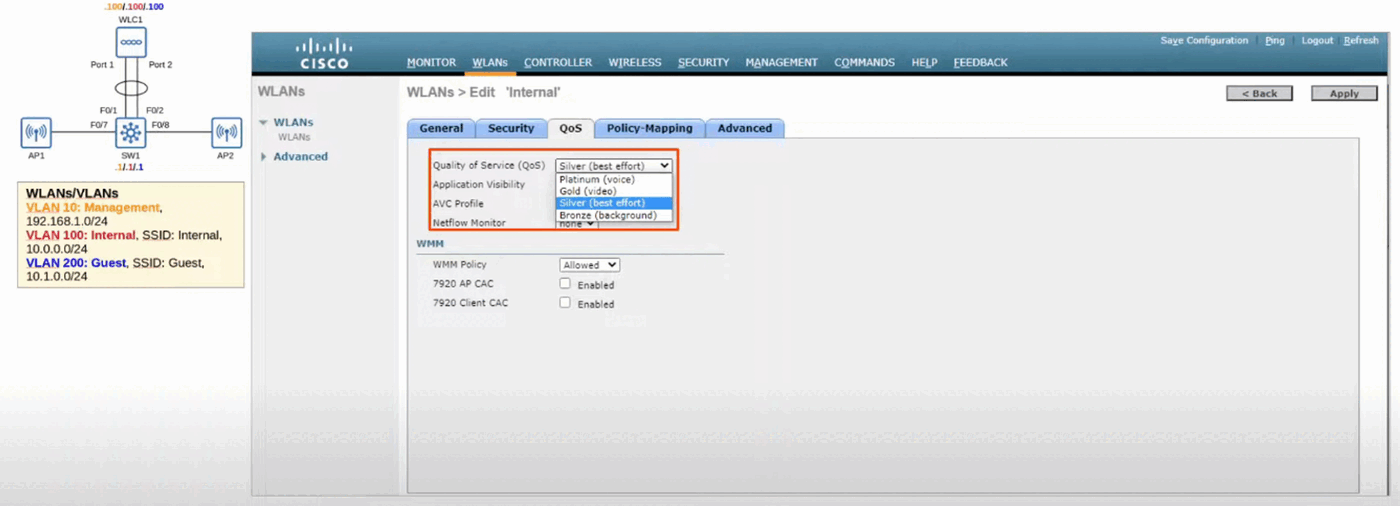
\includegraphics[keepaspectratio,alt={image}]{images/61-wireless-configuration/img-030.png}}
\end{figure}

Default QoS setting is ``SILVER'' (Best Effort). This can be changed
depending on the class of traffic being sent through the WLAN

\section{Advanced Settings}\label{advanced-settings}

\begin{figure}
\centering
\pandocbounded{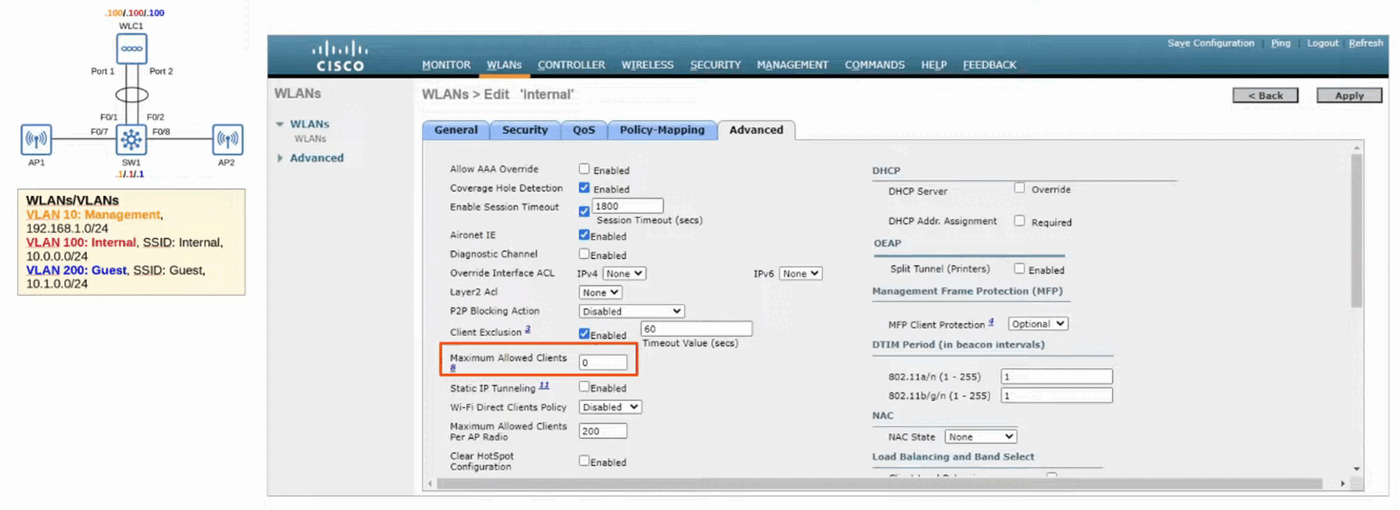
\includegraphics[keepaspectratio,alt={image}]{images/61-wireless-configuration/img-031.png}}
\end{figure}

\begin{figure}
\centering
\pandocbounded{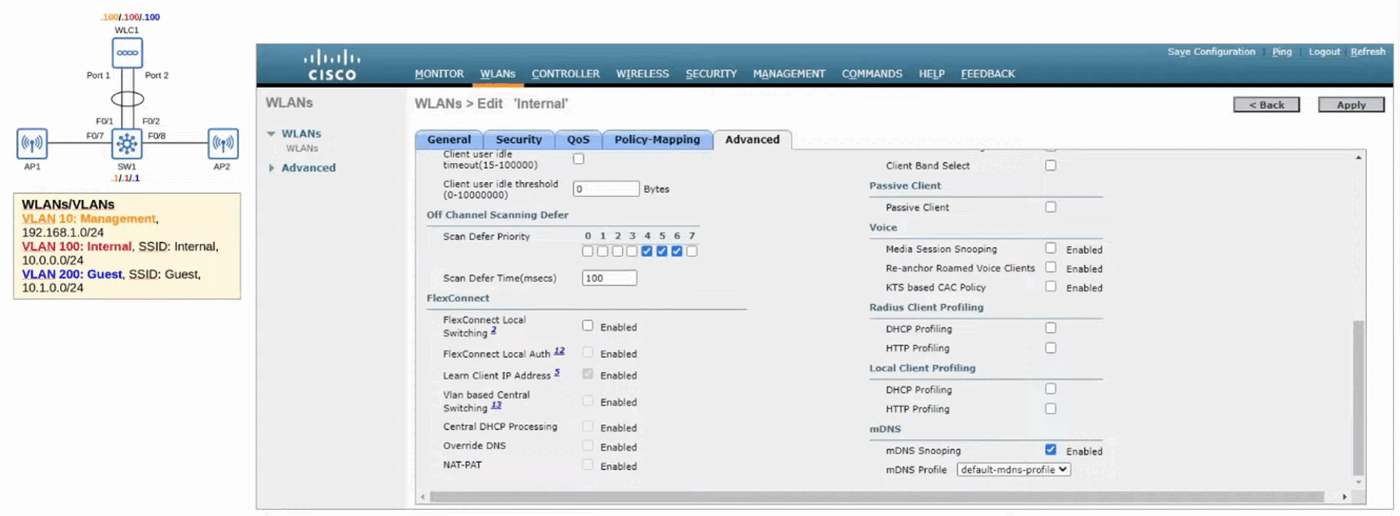
\includegraphics[keepaspectratio,alt={image}]{images/61-wireless-configuration/img-032.png}}
\end{figure}

\section{Configuring a New WLAN
(Guest)}\label{configuring-a-new-wlan-guest}

\begin{figure}
\centering
\pandocbounded{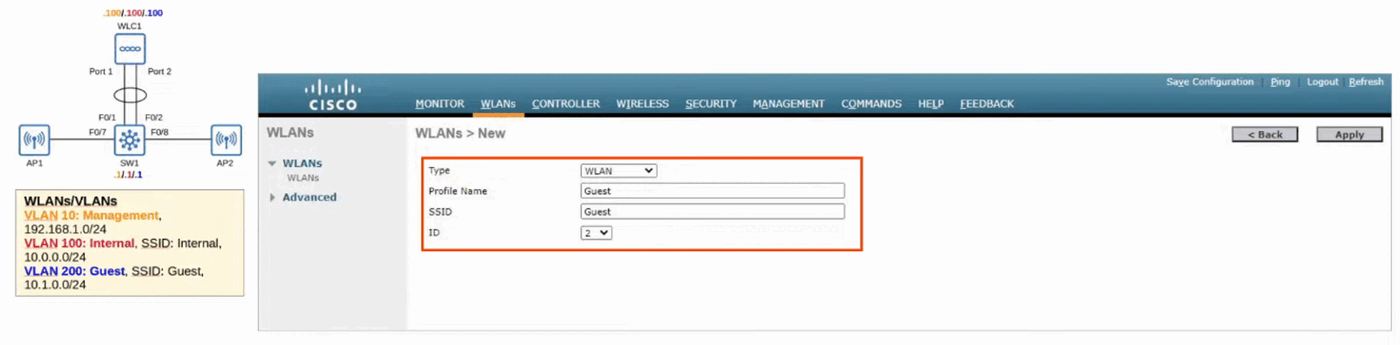
\includegraphics[keepaspectratio,alt={image}]{images/61-wireless-configuration/img-033.png}}
\end{figure}

Change STATUS to ``ENABLED'' and INTERFACE GROUP to ``GUEST''

\begin{figure}
\centering
\pandocbounded{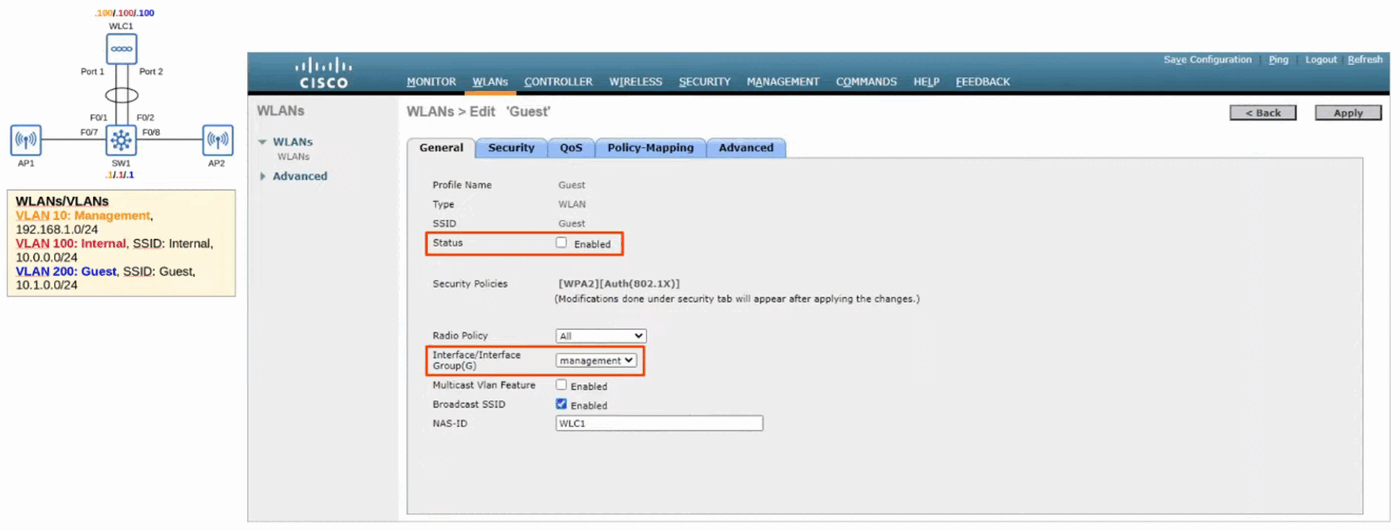
\includegraphics[keepaspectratio,alt={image}]{images/61-wireless-configuration/img-034.png}}
\end{figure}

\begin{figure}
\centering
\pandocbounded{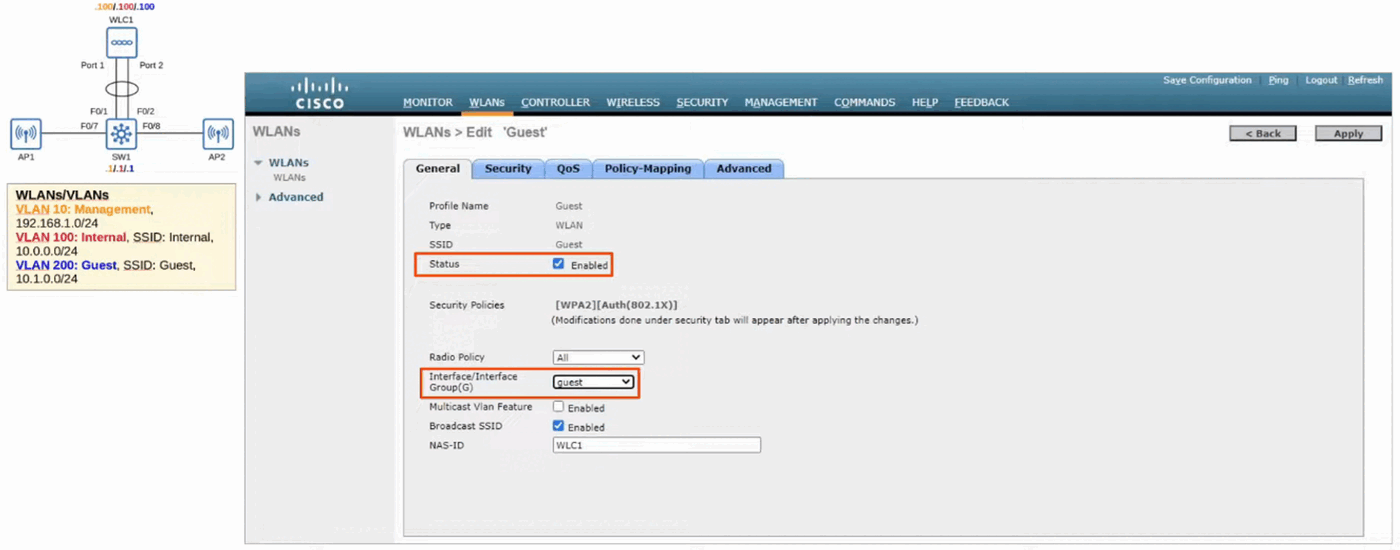
\includegraphics[keepaspectratio,alt={image}]{images/61-wireless-configuration/img-035.png}}
\end{figure}

Now, we need to change the SECURITY POLICY to {[}WPA2{]}{[}Auth(PSK){]}

Returning to MONITORING, we can see the changes we made to the
CONFIGURATION

\begin{figure}
\centering
\pandocbounded{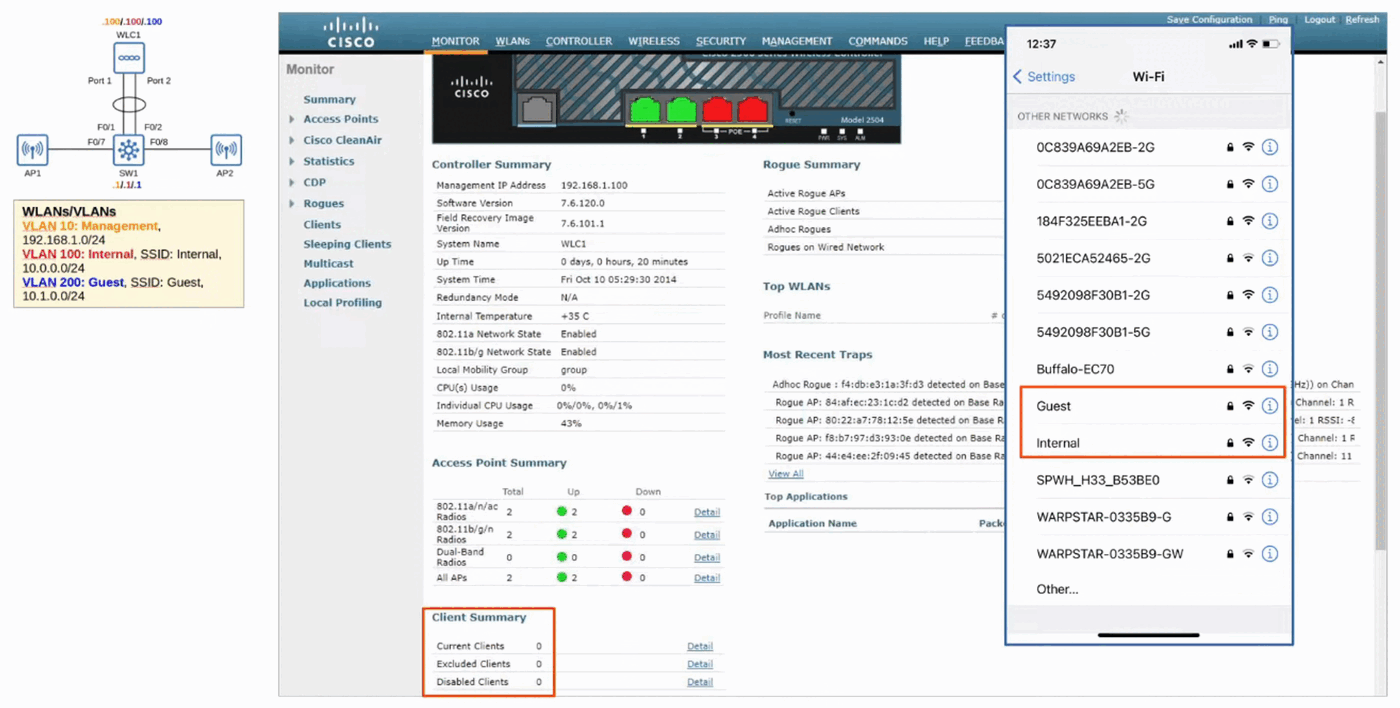
\includegraphics[keepaspectratio,alt={image}]{images/61-wireless-configuration/img-036.png}}
\end{figure}

Current number of CLIENTS is now 0. By connecting to the WLANS, these
numbers should change. To SEE a list of the CLIENTS connected, click the
left-hand side ``CLIENTS'' tab

\begin{figure}
\centering
\pandocbounded{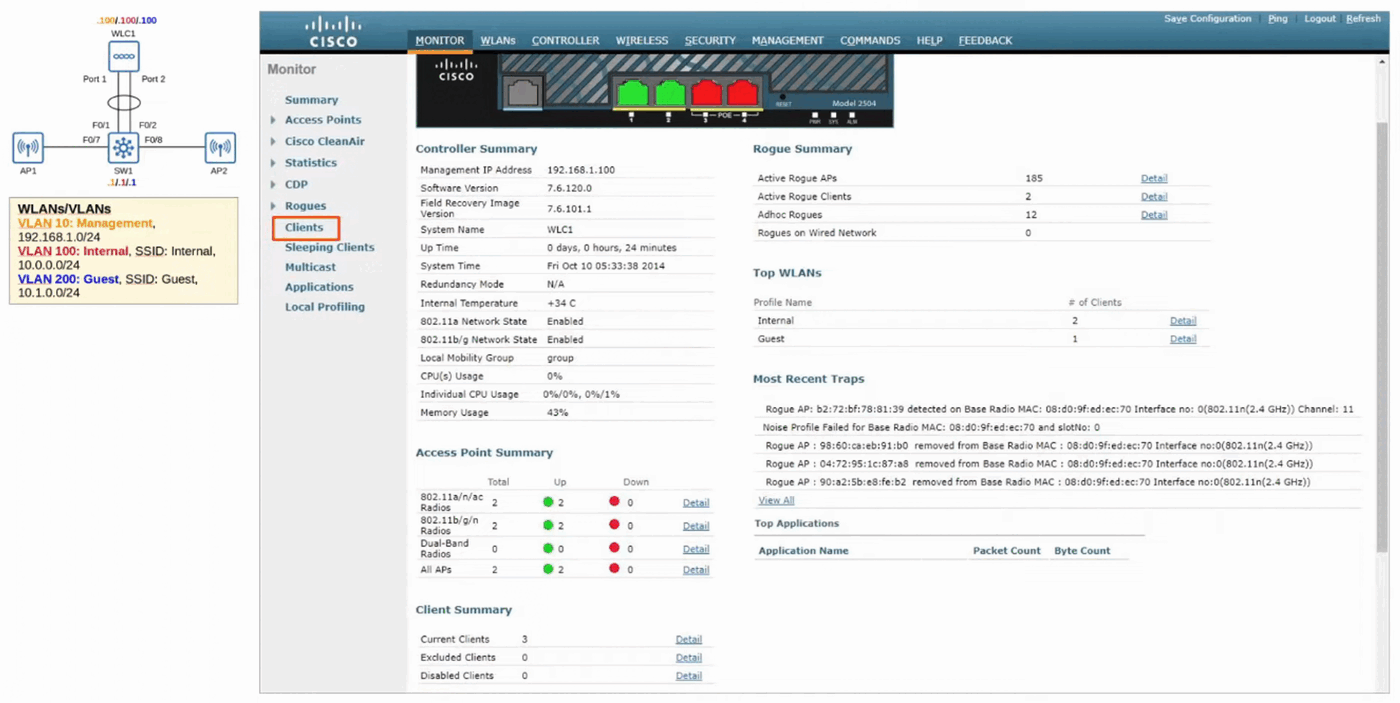
\includegraphics[keepaspectratio,alt={image}]{images/61-wireless-configuration/img-037.png}}
\end{figure}

\begin{figure}
\centering
\pandocbounded{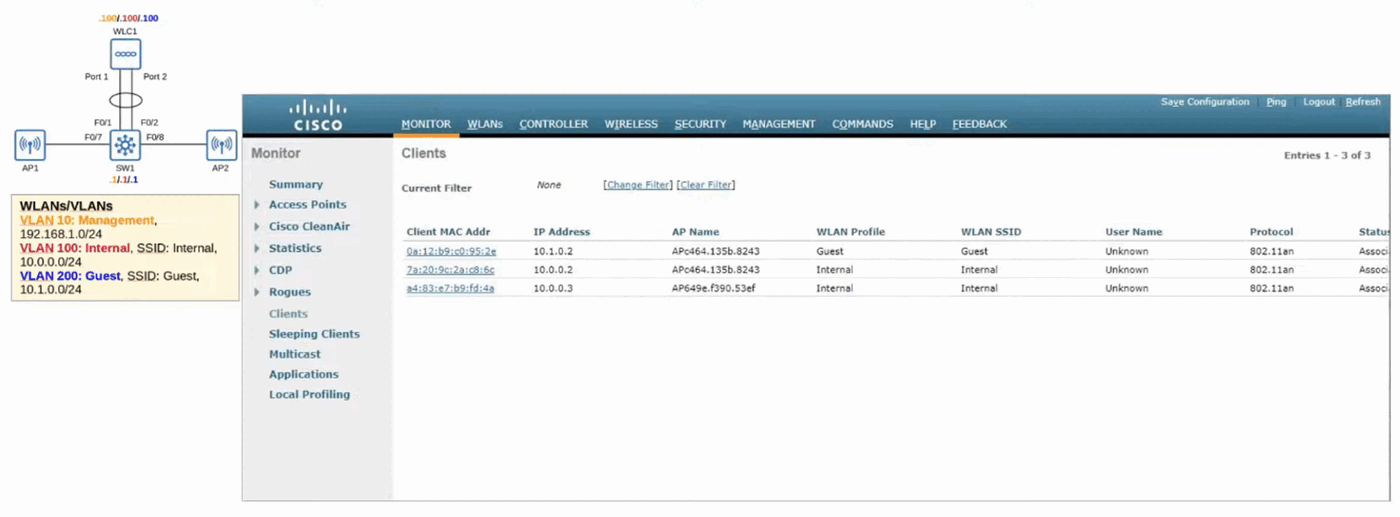
\includegraphics[keepaspectratio,alt={image}]{images/61-wireless-configuration/img-038.png}}
\end{figure}

\section{Addtional WLC Features}\label{addtional-wlc-features}

WIRELESS tab showing a list of the APs currently in the NETWORK

\begin{figure}
\centering
\pandocbounded{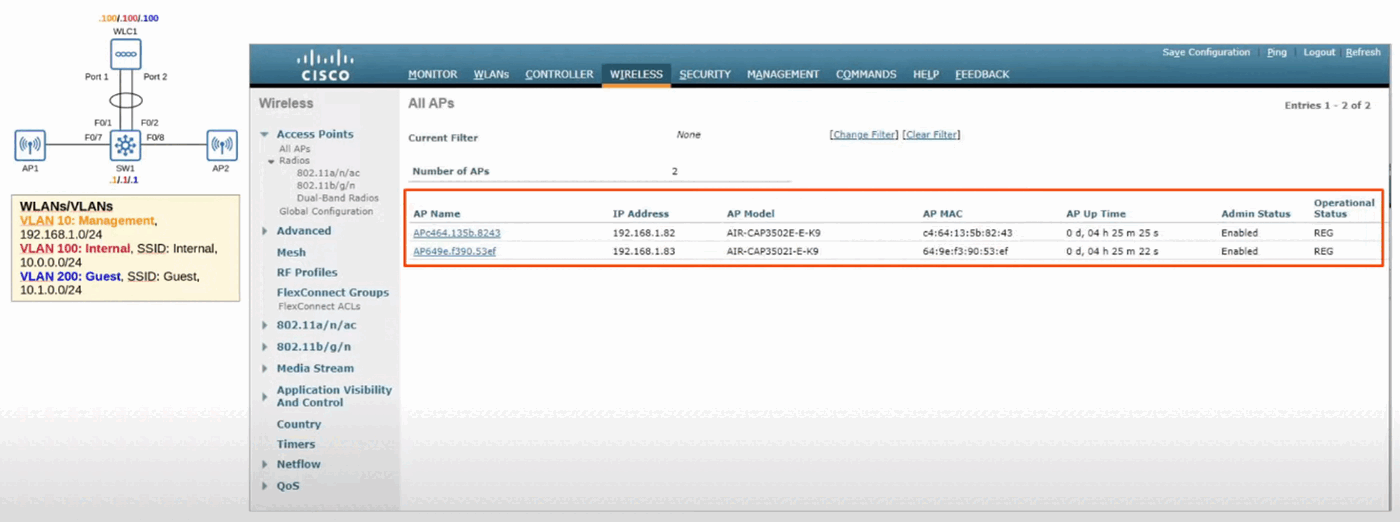
\includegraphics[keepaspectratio,alt={image}]{images/61-wireless-configuration/img-039.png}}
\end{figure}

Clicking on an AP shows information and configuration settings for it

\begin{figure}
\centering
\pandocbounded{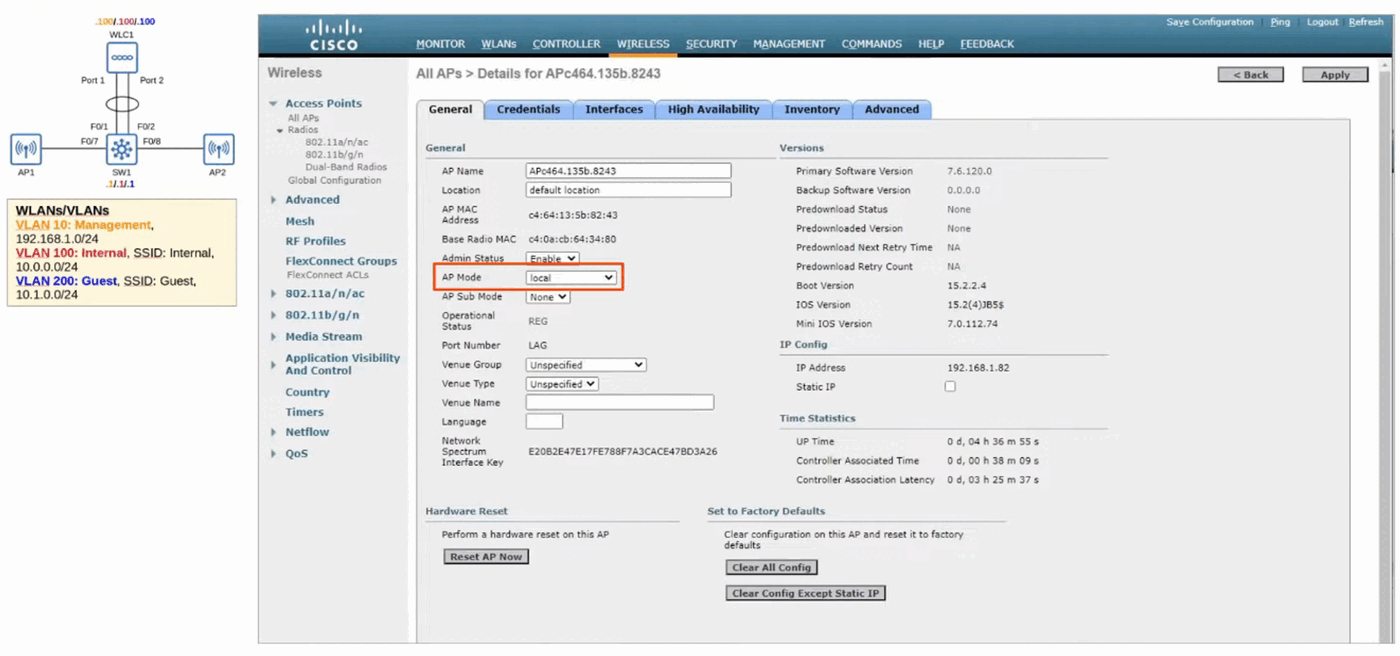
\includegraphics[keepaspectratio,alt={image}]{images/61-wireless-configuration/img-040.png}}
\end{figure}

MANAGEMENT tab allows you change the ways you can MANAGE the WLC

Clicking ``Mgmt Via Wireless'' allows you change if you can access
MANAGEMENT via WI-FI

\begin{figure}
\centering
\pandocbounded{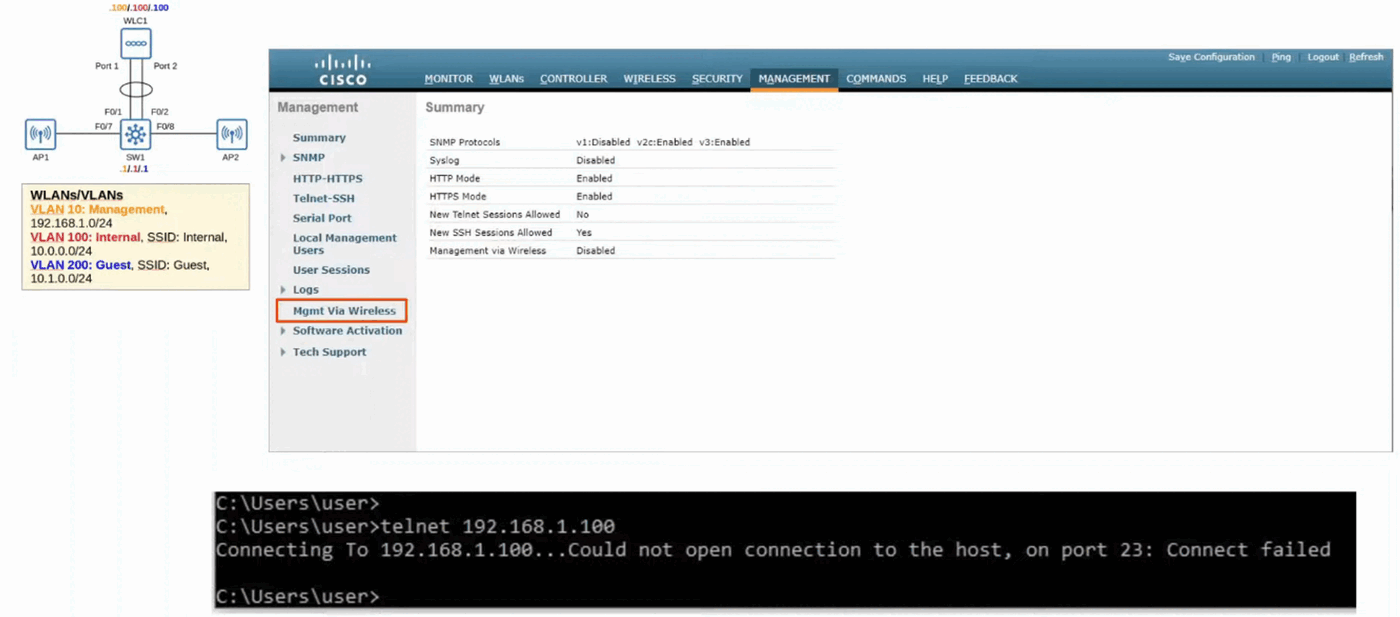
\includegraphics[keepaspectratio,alt={image}]{images/61-wireless-configuration/img-041.png}}
\end{figure}

\begin{figure}
\centering
\pandocbounded{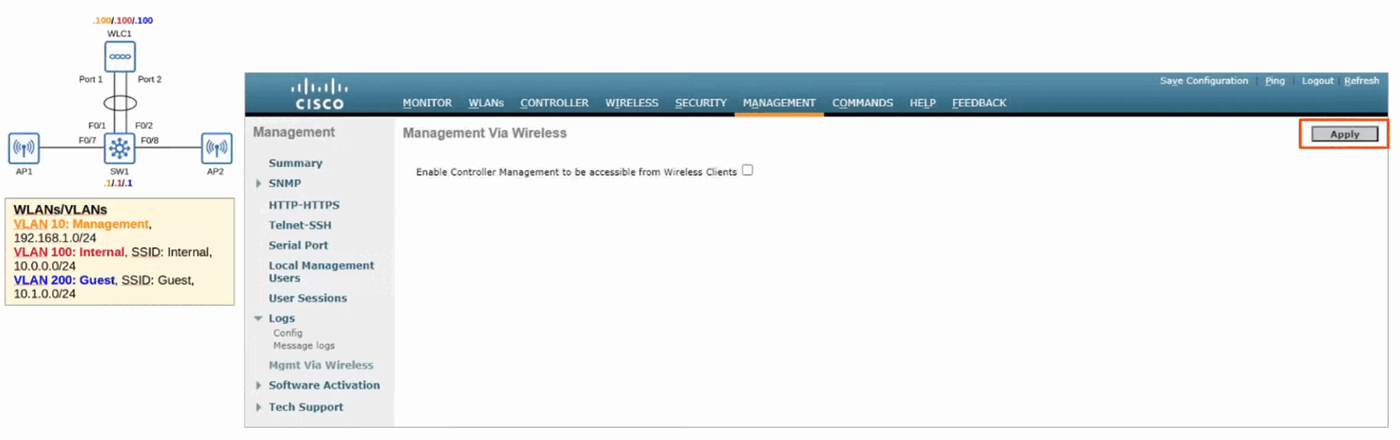
\includegraphics[keepaspectratio,alt={image}]{images/61-wireless-configuration/img-042.png}}
\end{figure}

SECURITY tab can allow us to create ACCESS LISTS

\begin{figure}
\centering
\pandocbounded{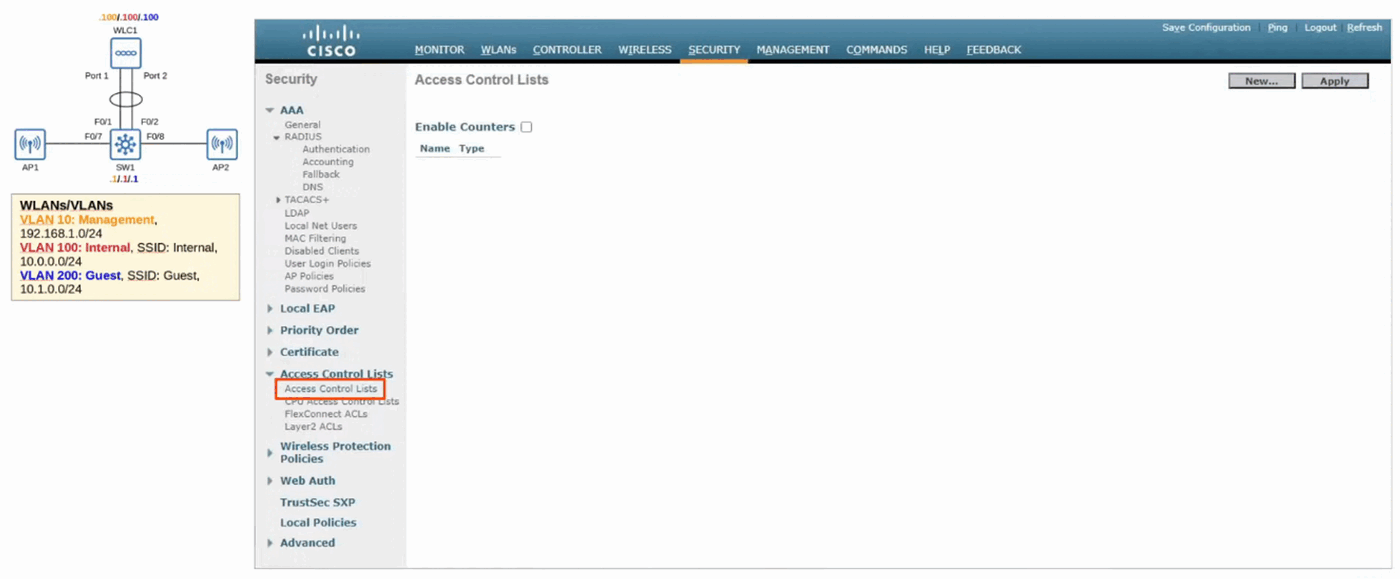
\includegraphics[keepaspectratio,alt={image}]{images/61-wireless-configuration/img-043.png}}
\end{figure}

First, NAME the ACL and what kind of IP ADDRESS it's for

\begin{figure}
\centering
\pandocbounded{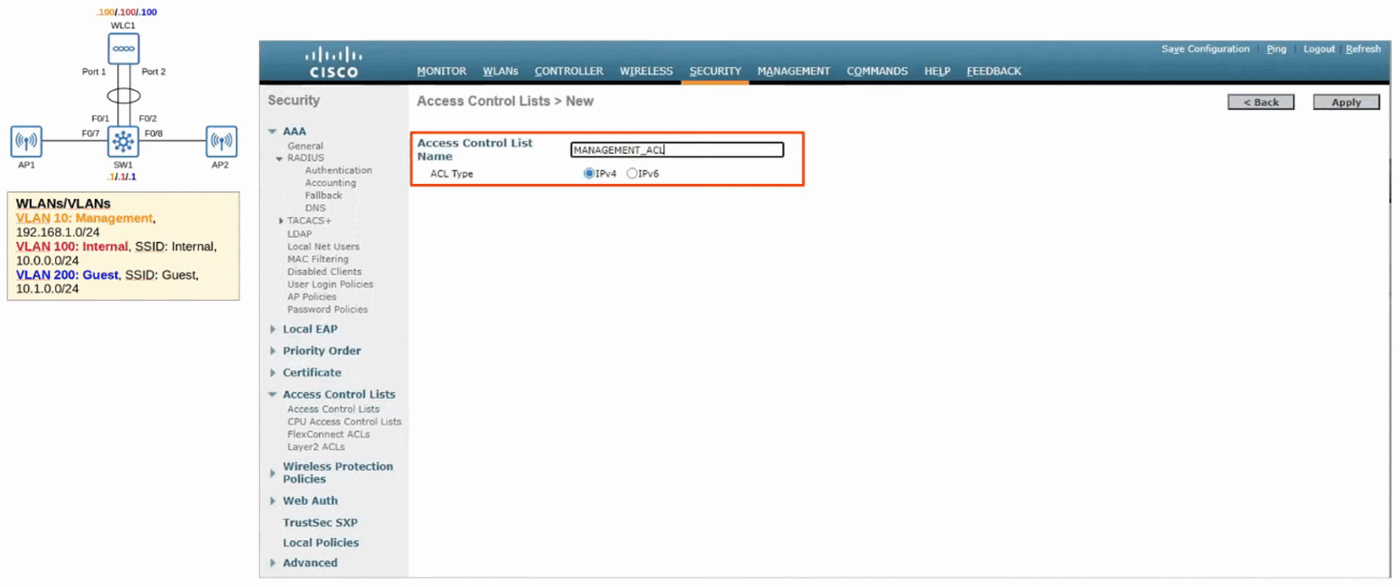
\includegraphics[keepaspectratio,alt={image}]{images/61-wireless-configuration/img-044.png}}
\end{figure}

CLICK ``Add New Rule'' to specify the ACL Rules (What traffic can pass)

\begin{figure}
\centering
\pandocbounded{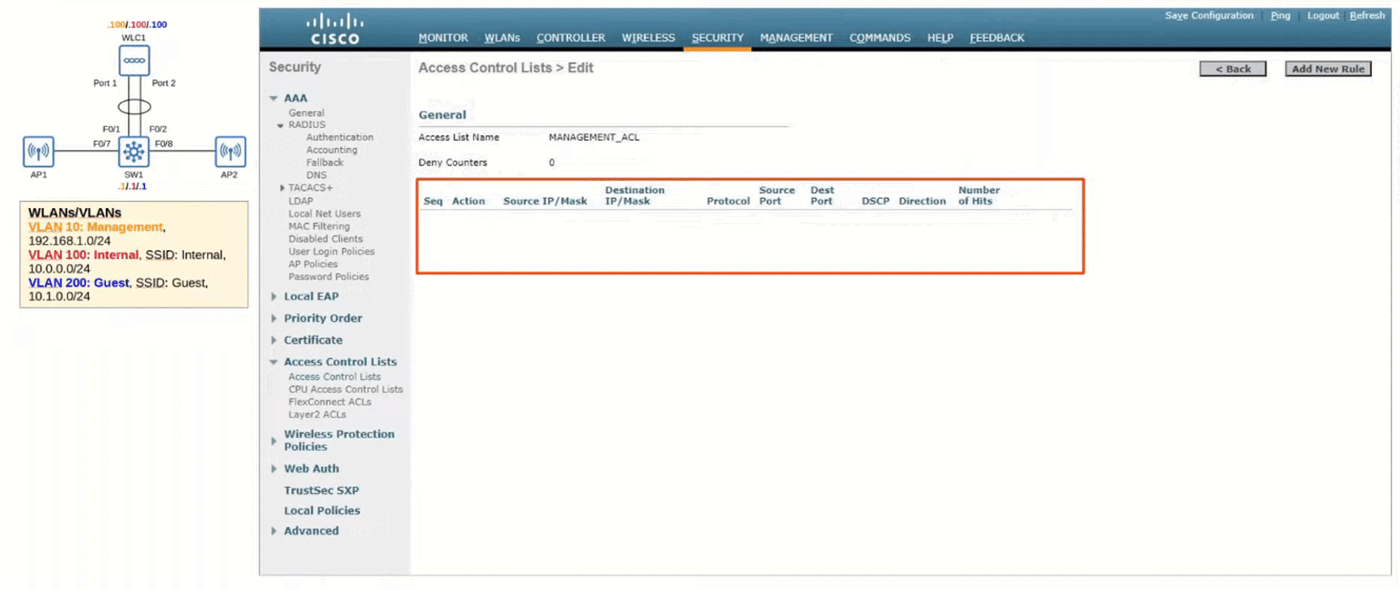
\includegraphics[keepaspectratio,alt={image}]{images/61-wireless-configuration/img-045.png}}
\end{figure}

\begin{figure}
\centering
\pandocbounded{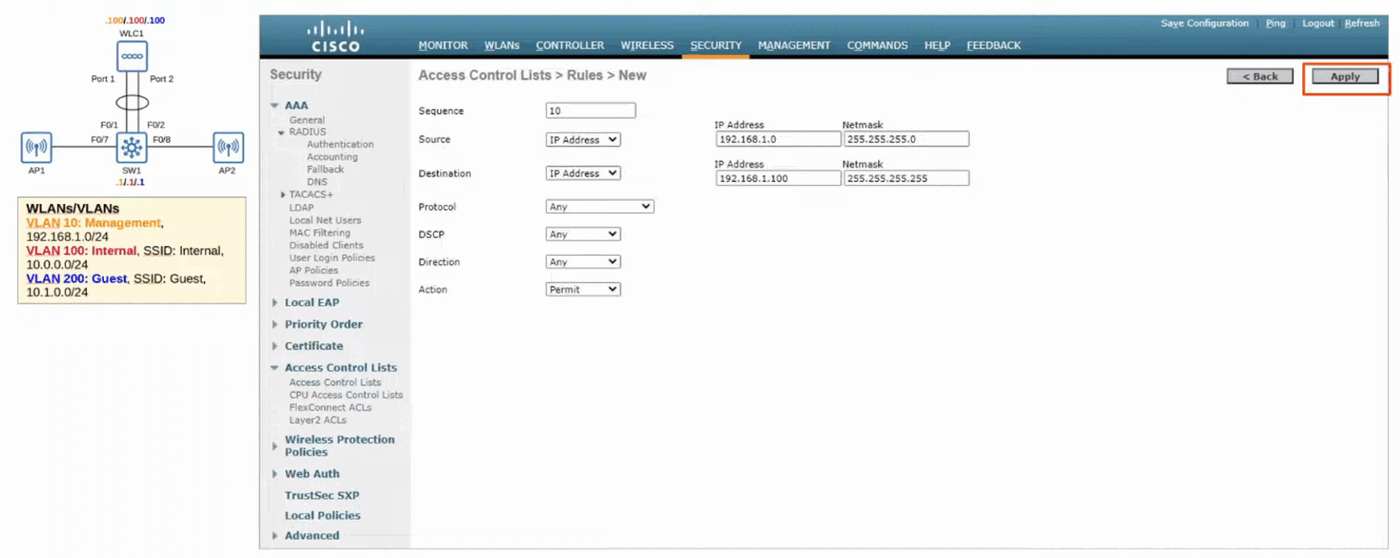
\includegraphics[keepaspectratio,alt={image}]{images/61-wireless-configuration/img-046.png}}
\end{figure}

\begin{figure}
\centering
\pandocbounded{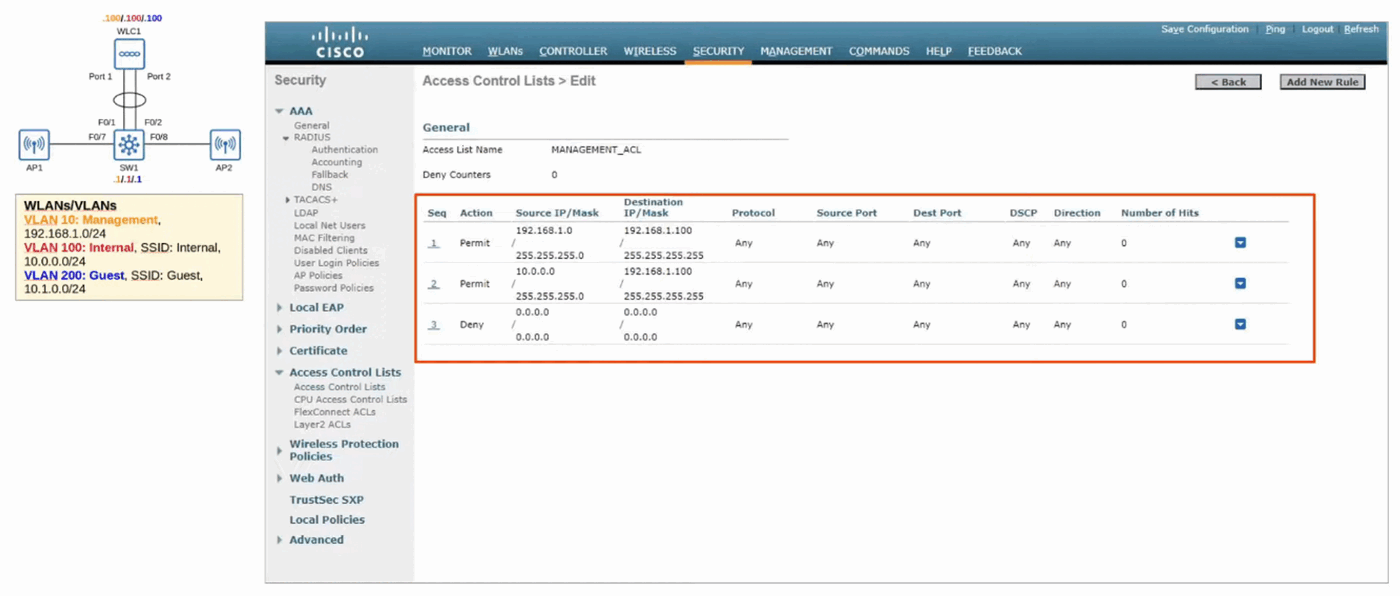
\includegraphics[keepaspectratio,alt={image}]{images/61-wireless-configuration/img-047.png}}
\end{figure}

We now need to APPLY the ACL (just like applying it to an INTERFACE on a
ROUTER)

Click ``CPU ACL'' from the left-hand menu

\begin{figure}
\centering
\pandocbounded{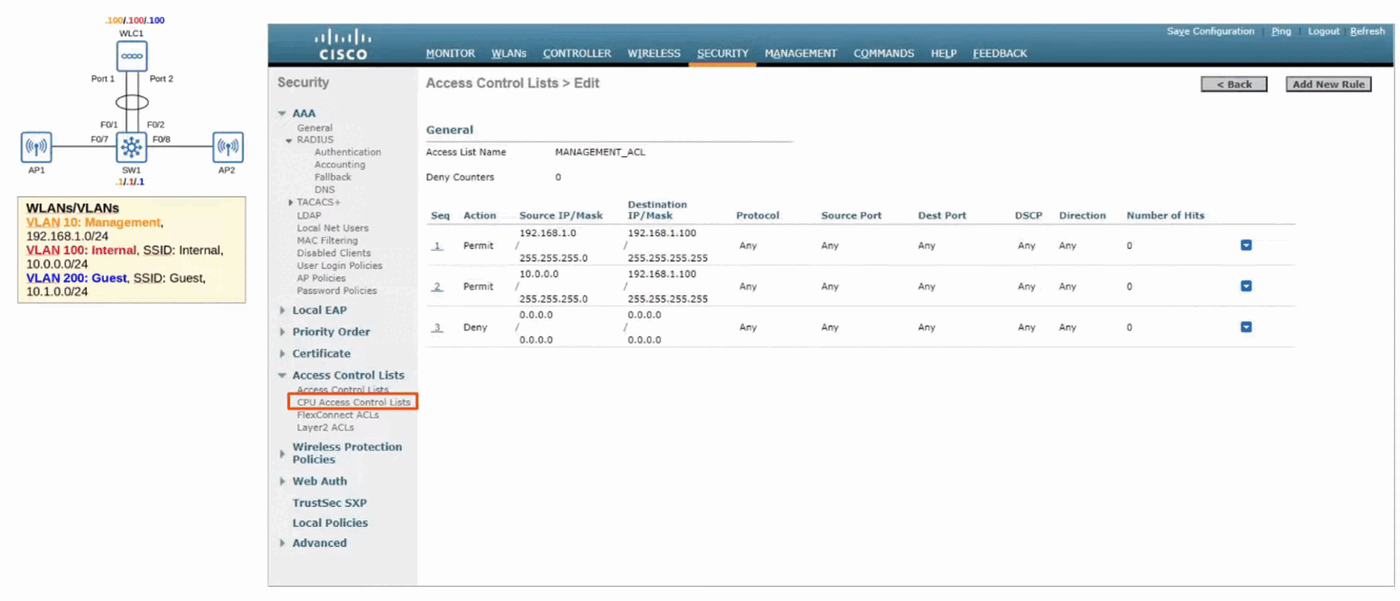
\includegraphics[keepaspectratio,alt={image}]{images/61-wireless-configuration/img-048.png}}
\end{figure}

Select the new ACL from the pull-down list and then click ``APPLY''

\begin{figure}
\centering
\pandocbounded{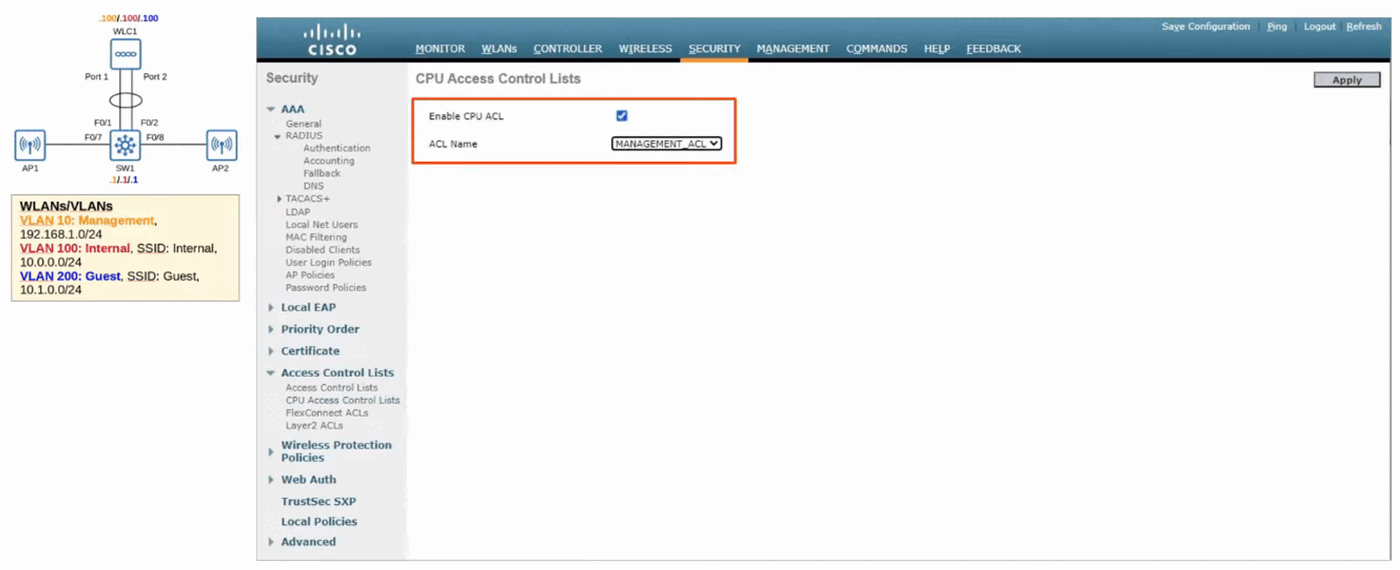
\includegraphics[keepaspectratio,alt={image}]{images/61-wireless-configuration/img-049.png}}
\end{figure}

\begin{figure}
\centering
\pandocbounded{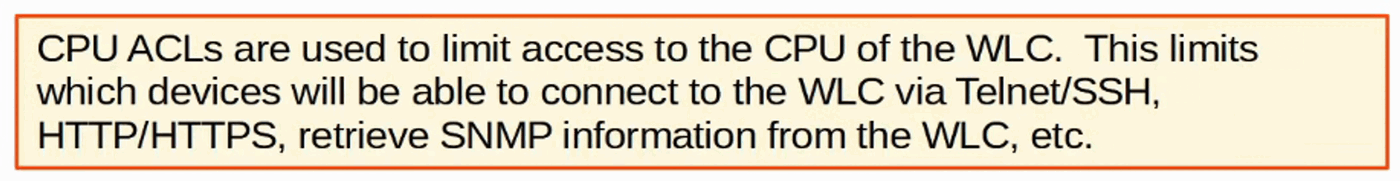
\includegraphics[keepaspectratio,alt={image}]{images/61-wireless-configuration/img-050.png}}
\end{figure}
